\section{ナノサイエンス・デバイス}
\label{sec:ナノデバイス_詳細}

\subsection{現在行われている課題}
半導体材料や高分子材料など、20世紀の科学技術研究の中で生まれた物質群は、100種類ほどの元素の無限とも言える組み合わせの中から見出され、特異な機能や新しい現象の発現を通して、現代社会の産業基盤を形成してきた。
これらの物質や材料をミクロな視点に立って研究する物質科学は、物性科学、分子科学、材料科学という三つの学問分野にまたがり、基礎研究と応用研究をつなぐ役割をも担う、広大な学問分野である。

物質科学分野における大規模数値シミュレーションは、古くはFermi-Pasta-Ulamの非線形励起・再帰現象、剛体球のAlder転移などの概念革新への寄与に始まり、現代量子多体系では、分数量子ホール効果の数値検証、相転移と臨界現象の解明、高温超伝導の機構提案など、物質科学の基礎研究に欠かせぬものとなった。
この分野では、電子状態を量子力学に基づいて第一原理的に計算する手法として、波動関数理論に基づいた量子化学計算や量子モンテカルロ計算、密度汎関数理論に基づいたバンド計算がある。
また、大規模な原子・分子系の集団運動を古典力学・統計力学に基づいて計算する古典分子動力学法、古典モンテカルロ法などの分子シミュレーションがある。
更に、物質を粗視化した連続体として扱う方法として、有限要素法やフェーズフィールド法がある。特に産業応用に直結する領域においては、単一の大規模ジョブだけでなく、アレイジョブ、すなわちパラメータサーチも重要となってきている。

物質科学分野においては、現在「次世代先端デバイス科学」、「分子機能と物質変換」、「エネルギー変換」、「マルチスケール材料科学」といった社会的にも重要な課題群に、それらの源流とも言うべき「新量子相・新物質の基礎科学」を加えた5つの課題が「京」コンピュータを用いて重点的に進められている。

\rmproject{次世代先端デバイス科学}
半導体テクノロジーはポストスケーリング時代を迎え、ナノドット、ナノワイヤーなどの構造体が次世代デバイスに不可欠な要素となっている。それらナノ構造体の構造的安定性と電子機能についての高精度の予測を目指し、主に密度汎関数法に基づくシミュレーション技術が確立されてきた。
海外では、ABINIT (白)・CASTEP(英)・CONQUEST(英日)・CP2K(欧)・CPMD(独)・QUANTUM ESPRESSO(伊)・SIESTA(西)・VASP(墺)・WIEN2K(墺)、また国内では、ASCOT・CMD・FEMTECK・OPEN-MX・PHASE・QMAS・RSDFT・TAPP・TOMBO・UVSORなど、それぞれ特色のあるコードが開発されている。
国内ソフトウェアでは、超並列計算の実績のあるものも多く、代表的なものとしては、「京」コンピュータで3PFLOPS(44\%の実効効率)を達成し2011 ACM Gordon-Bell Prizeを受賞したプログラムRSDFT、初代地球シミュレータ 512ノード(4096CPU)で50\%の実効効率を出したプログラムPHASE(12,288原子系を「京」12,288ノードで23\%の実効効率)などがある。
これらの高度に最適化・高速化されたソフトウェアにより、1,000〜100,000原子規模のナノワイヤーの電子状態や伝導特性の計算、1,000,000原子規模のGeナノ構造の解明などが進んでいる。

一方、実在系ナノ構造体を対象とした光・電子デバイスの第一原理計算に基づく理論設計の試みは、現状では国内外ともにほぼ皆無と言ってよいが、わが国ではデバイス設計に不可避である光と物質の露わな相互作用を取り込んだナノ光学理論に基づく電子・電磁場ダイナミクス法プログラムが、「京」コンピュータ24,576ノードでの実機稼働に成功しており、十数ナノメートル程度のナノ構造体の電子・電磁場ダイナミクスであれば十分に計算可能な状態となっている。
今後、2016年までの間に更なる超並列化を行い、実在系ナノ分子構造体を対象とした光・電子デバイス設計に展開する。

\rmproject{分子機能と物質変換}
分子や分子集団系における構造形成と機能発現・機能制御の分子科学の確立を目指して、自己組織化により形成されるナノスケールの分子・分子集団の構造に基づき創成される機能の解明、環境との相互作用下での分子の電子状態に立脚した機能発現メカニズムの解明などが進んでいる。
計算科学的手法としては、古典分子動力学法、自由エネルギー計算、FMOや分割統治法に基づく量子化学計算、およびそれらを組み合わせた、QM/MM法、ONIOM法、レプリカ交換法などが用いられている。

分子動力学計算においては、国内外でさまざまな競合ソフトウェアが開発されている。国外ではAMBER(米)・CHARMM(米)・DESMOND(米)・GROMACS(蘭)・LAMMPS(米)・NAMD(米)・TINKER(米)、国内ではMARBLE・MODYLAS・MPDYN・PEACH・PLATYPUSなどがあり、非常に多岐にわたる。
その中でも日本発の長距離古典分子動力学計算プログラムMODYLASは、長距離相互作用計算に高速多重極展開法を導入し、更に隣接通信を最適化することにより「京」65536ノードで実行効率41.1\%、並列化効率80.9\%を達成した。
更にウイルスとレセプターからなる1000万原子系に至る巨大系にMODYLASを適用し、生体のウイルス認識の分子論を展開している。

\rmproject{エネルギー変換}
化学結合エネルギー、電気エネルギー、太陽光、熱エネルギーの間の相互変換における物質の機能の役割を明確化し、エネルギー変換の大幅な高効率化につなげるための計算手法の開発、コード開発、シミュレーションが進められている。
燃料電池やリチウムイオン2次電池における電気化学過程、色素増感型の太陽電池の界面構造などの研究には、主として大規模な第一原理分子動力学計算が用いられている。
また、水素・メタンハイドレートの熱力学過程の解明には古典分子動力学法などが、バイオマス利用における酵素反応の解明には有効媒質法(3D-RISM法)などが有効である。
わが国においては、いずれのシミュレーション手法についても大規模並列環境への最適化・高度化が進んでおり、理論的な蓄積と合わせて国際的にも優位な立場にある。

\rmproject{マルチスケール材料科学}
実用材料の飛躍的高性能化に向けて、マルチスケールシミュレーションで材料組織を設計し、評価する試みが進んでいる。
一例として、高精度の自由エネルギー計算による相図計算、各相の自由エネルギーや界面・粒界・欠陥の第一原理計算と、フェーズフィールド法・分子動力学計算・モンテカルロ法などとの連結が挙げられる。
これらの連成計算では、各スケールの計算規模はそれほど大きくないものの、それらを効率的に組み合わせて実行する必要がある。
下部計算となる第一原理計算では、ABINIT・QMAS・TOMBO・OPEN-MXなど国内外で開発されたさまざまなソフトウェアが対象に応じて使い分けられる。
第一原理計算の結果を用いた上部計算(分子動力学計算)を行うFERAMなどのソフトウェアも開発され、広く使われている。

\rmproject{新量子相・新物質の基礎科学}
粒子間の相互作用の強い分子系や凝縮物質を取り扱う強相関多体量子科学・計算科学の汎用的手法の開発が進み、新奇な量子多体現象の発見と機構解明、新しい量子機能を持つ新物質の探索、化学反応や分子集団の非平衡ダイナミクスの理解を目指して研究が進められている。

強相関量子多体系のモデル計算については、厳密対角化や密度行列繰り込み群(DMRG)、変分モンテカルロ法や世界線量子モンテカルロ法などさまざまな手法により、鉄系超伝導体・銅系超伝導体の機構解明、強相関電子系のダイナミクスの解明、新しい量子臨界現象の解明などが進んでいる。
国内においては、「京」24,576ノードでピーク性能比10\%以上を達成した変分モンテカルロ法MACE/mVMC、ピーク性能比で70\%を達成した動的密度行列繰り込み群法DDMRGなど、大規模並列環境への最適化も進んでいる。
この分野は手法自体の発展が速く、コミュニティーコードと呼ばれるものは、まだ十分に育ってきているとは言えないが、ALPSなど量子格子模型に対するソフトウェアパッケージの開発も進みつつある。
その中でも世界線量子モンテカルロ法ALPS/looperは、非局所グラフ操作など従来の計算機が不得手とする演算が主体であるにもかかわらず、「京」24,576ノードでMIPSピーク性能比10\%以上の性能を達成している。

一方、量子化学計算については、ADF(蘭)・GAUSSIAN(米)・GAMESS(米日)・NWCHEM (米)・MOLCAS(典)・MOLPRO(独)・QCHEM(米)・TURBOMOLE(独)など欧米各国では一般ユーザにも使いやすい汎用コードの開発が進んでいる。
日本においてもABINIT-MP(X)・GELLAN・OPEN-FMO・NTCHEM・PAICS・PROTEINDFなどが開発されている。しかしながら、超並列環境への対応は十分とは言い難い。
しかしながら、国内で開発されている量子化学計算プログラムGELLANは、超並列機に対する最適化が進んでおり、「京」24576ノードで実行効率28\%、並列化効率80\%を達成した。
更に、ほぼ基底関数極限での露わに相関した2次の摂動法でC60フラーレン2量体の相互作用エネルギーの計算を行い、ナノスケール分子系の超高精度計算が実現可能になったことを示した。

このように、物質科学全般において、国内外で超並列環境に最適化された大規模ソフトウェアの開発が進められている。
一方で、基礎理論自体が多層構造をなしており、それぞれのレベルにおける方法論が非常に多岐にわたり、かつそれぞれが相補的に発展してきたことが、物質科学のもう一つの大きな特徴である。シミュレーションの大規模化・精密化を進めると同時に、全く新しい基礎理論・モデルの提唱、シミュレーション手法の開発・実装・高度化、最先端の計算機を使ったシミュレーションによる予言・検証と理論へのフィードバックというサイクルを効率よく進めていくことが、今後の計算物質科学分野の発展のために重要である。

\subsection{長期的目標}
物性科学は$10^{23}$ほどの膨大な数の原子、分子多体系から成る自然を理解する営みを通じて、相転移にともなう自発的対称性の破れ、集団運動励起やトポロジー励起、マクロ量子現象といった基礎科学を一新する普遍概念をもたらし、素粒子物理学から経済学まで広がるさまざまな学問分野に大きな影響を与えてきた。

分子科学は、化学反応の理解とそれに基づく新しい分子・分子集合体の創製を通じて、物質科学研究に大きな展開をもたらしてきた。

材料科学は、一辺の長さが原子10個分くらいに相当するナノメートルのスケールで物質材料を捉えることにより、金属組織や粒界、複合材料など、材料としての利用に係る諸問題の解決を目指してきた。

これらの成果は、20世紀以降の産業・先端技術革新を生み出す基盤となった。トランジスタ、トンネルダイオード、半導体レーザー、集積回路、巨大磁気抵抗素子、CCD(電荷結合素子)、有機ELなどの革新デバイス、合成樹脂や導電性高分子などの新材料は、ノーベル賞の受賞対象ともなった物質科学の基礎研究が生んだ例である。
同じく物質科学の精華である超伝導は、最先端の医療用MRIの超伝導マグネットに使われ、更に超伝導リニアモーターやエネルギー損失のない電力線として実用化されようとしている。高効率の太陽電池や高効率熱電素子など、地球規模のエネルギー問題解決に向けた新しい概念に基づくデバイスも、物質科学の基礎研究に基づいて提案され始めている。
燃料電池に用いられる白金触媒、色素増感太陽電池に用いられるルテニウム、透明電極に使われるインジウム、リチウムイオン電池材料のリチウムやコバルトなど供給量が希少、あるいは今後の需要増に応じて希少になると考えられる元素の代替材料を他国に先駆けて開発することが、わが国の産業競争力を高めるためにも必要である。

一方、原子の組み合わせからさまざまな官能基・分子ができ、その多様な組み合わせで、溶液・ミセル・脂質膜・タンパク質・高分子・クラスレートハイドレートなどが形成される。
これらの系では、環境の熱エネルギー程度の弱い相互作用の制御によって、分子の認識、分配、分離、輸送といった多様な機能を制御・設計することができ、ドラッグデリバリーシステム(drug delivery system; DDS)、高分子分離膜(海水淡水化等)、食品・コスメティック、生体模倣材料、化学工学プラント設計、ガス分離、温暖化ガスの吸収、電池電解液、結晶成長といった広範な学術的・社会的ニーズに直結する。

界面系では、凸凹があり不純物も存在する現実系の取り扱いが可能になりつつある。分子素子やナノテクノロジー・トライボロジーの新展開の場であり、環境科学との関連も深い。

20世紀の要素解明から21世紀には集団・階層解明と機能制御の時代に入ったと言われる現代科学の中核として、物質科学における基礎研究のフロンティアでは、量子ホール効果、トポロジー絶縁体、スピン液体、量子臨界や脱閉じ込めといった新概念が次々に発見され、自然の新たな機構解明への挑戦が続けられている。
概念の革新は次世代、次々世代の最先端技術へ展開する研究をますます活性化させているが、この基礎研究から応用研究、更には産業応用への多段階リレーは、高度な蓄積を持つわが国を含むきわめて限られた国でのみ追求し得る。

更に近年、高性能のスパコンを活用することで、近代までに確立された古典力学、量子力学、統計力学に基づいた、ナノ材料の物性・化学のボトムアップ的な予測に期待が寄せられている。

計算科学と実験・理論がタイアップし、次世代の半導体デバイス、触媒材料、各種電池、薬剤、触媒などの設計・開発に役立てることで、地球環境を守り、産業振興を助け、社会を豊かにすることにつなげることができる。

\rmproject{次世代先端デバイス科学}
現有の半導体電子デバイスをベースとして更に高機能化したものは、次世代量子デバイスの有力候補の一つになると予想されるが、その一方で高機能化半導体電子デバイスの実現に際しては、微細化、高速化、大容量化、低消費電力化、熱対策等、解決すべき非常に大きな障壁があることも事実である。
これらの問題に対して相補的な、あるいは理想的には根本的な解決策を与え、更には電子デバイスにはない高機能性を備えた次世代量子デバイスの一つの候補として、ナノ分子構造体を利用した光・電子機能性デバイスが考えられる。
分子の持つ合成設計柔軟性と構成原子の多様性に起因する高機能発現能力を最大限に利用したナノ構造体において、光と電子のダイナミクスの二つの自由度が結合することによってこれまでとは本質的に異なる機能が発現すると期待できる。
今後はこのようなナノ分子構造体を使った光・電子機能性デバイスの理論設計を積極的に進める。
このため、「京」コンピュータで開発された電子・電磁場ダイナミクス法プログラムを更に超並列化することにより、デバイスの理論設計を加速させる。

本研究の中核であるナノ光学理論が完成すれば、従前の光学応答現象を大きく超えた理学・工学の新たな研究領域を切り開くことが期待でき、その学術的意義は非常に高い。
また、これらはいずれも次世代量子デバイス設計原理に大きく関わる現象であり、計算科学を通じて「ものづくり」の観点から社会へ大きな還元ができると考える。

\rmproject{分子機能と物質変換}
物質変換技術は、基盤産業の基礎であるとともに、人類の生活を豊かにした科学技術という点で最も成功した技術であると言える。

分子と化学反応の微視的理解に基づいて、さまざまなクロスカップリング反応のような精密有機合成反応、バイナップなどの使用による高立体選択的合成反応、重合反応や脱硝、脱硫反応など、新しい考え方による物質変換反応が次々に開発されてきた。
衣類、家や車の構造物、更には液晶や有機ELのような電子材料、航空機の構造材料など、化学反応による物質変換の成果は枚挙にいとまがない。
今後のわが国の産業競争力を更に強化し、地球規模での資源問題を解決するためには、目的の物質を安価で汎用的な材料から効率よく作り上げることが不可欠である。
複雑な構造を持つ新しい有機分子触媒、金属微粒子、金属(酸化物)表面、金属錯体などをまるごと精密に計算することにより、分子の相互作用と化学反応過程を解明し、新しい物質変換法を理論先導的に開発することを目指す。

\rmproject{エネルギー変換}
エネルギー問題はわが国の最重要課題の一つであり、エネルギー資源小国であるわが国が世界の中でこれまで以上の繁栄を目指すためには、あらゆる科学技術を駆使してエネルギー創成・変換・利用技術を他国の追随を許さないレベルにまで高める必要がある。
そのためには、世界最高水準のわが国のエネルギー関連技術を科学にまで高め、試行錯誤というレベルとは異なる次元から物質開発を行うための道筋をつけることが必須である。

燃料電池や2次電池、太陽電池、あるいはバイオマス利用における電気化学過程、非平衡電気伝導などに対し、超並列大規模計算機を利用した第一原理に立脚したシミュレーション技術をかつてない高いレベルに押し上げる。
これにより、物質とエネルギーの関連を理論とシミュレーションから突き詰めて考え、次世代の高効率エネルギー変換に寄与する物質・材料開発に資する知見を獲得し、その成果を社会全体へと還元する。

\rmproject{マルチスケール材料科学}
熱エネルギーを効率的に機械・電気エネルギーに変換する耐熱材料や低燃費・省エネルギーに寄与する高比強度軽量材料等の飛躍的高性能化が、エネルギー問題の解決に向けて求められている。
こうした材料の強度・信頼性は、ミクロの原子間結合のみならず、メゾスケールの内部組織(析出相・粒界・異相界面・転移・点欠陥・不純物偏析等の集合体)に支配され、それらを系統的に設計・制御することが肝要である。
そのために、第一原理による電子構造計算やエントロピーを考慮した自由エネルギー計算、更にミクロからメゾ、マクロをつなぐマルチスケール計算が必須となる。

超並列大規模計算機環境を用いて、大規模第一原理計算・自由エネルギー計算を実行するとともに、フェーズフィールド法等により、ミクロ-メゾ-マクロをつなぐマルチスケール計算技術を確立し、内部組織の安定性、微細構造、強度、諸特性を解明する。(図\ref{fig:4-2_1})

\begin{figure}[H]
  \centering
  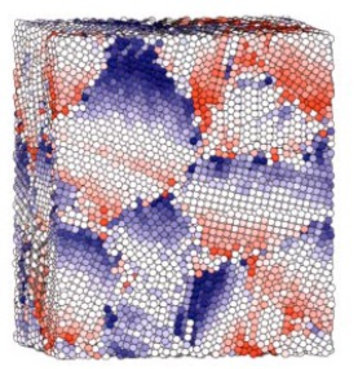
\includegraphics[width=0.3\textwidth]{figs/4-2_1.pdf}
  \caption{鉄の内部組織}
  \出典{○○○○○(香山正憲(AIST))}
  \label{fig:4-2_1}
\end{figure}


\rmproject{新量子相・新物質の基礎科学}
多体量子系の示す多様性や階層性の理解は、今世紀凝縮系科学の中心課題であり、人類の自然探索と理解の最前線でもある。
とりわけ、強相関多体量子系は新しい現象と概念の宝庫であり、高温超伝導、巨大応答、トポロジーで分類される量子ホール相やトポロジカル絶縁体などの物理を生み出し、遷移金属酸化物、希土類化合物、有機導体などの強相関電子物質群やナノチューブなどのクラスター化合物、量子ドットなどの微細加工構造、冷却中性原子などの新しい系の探索と理解へと導いた。

更なる進展のためには、物質科学の中核と基礎科学を担い、物理と化学の枠を超えて粒子間の相互作用の強い分子系や凝縮物質を取り扱う強相関多体量子科学・計算科学の汎用手法を確立し、多体集団の励起状態や非平衡ダイナミクスに対する飛躍的な理解を図る必要がある。
これにより、新しい量子相(新超伝導、新絶縁体、新量子液体)、すなわち、人類の知らない物質の新たな形態の発見を可能にするとともに、高温超伝導・高効率熱電素子・マルチフェロイクスなどの強相関新物質を次世代の応用や産業基盤開拓の基礎として展開していく。

また、高精度電子相関理論の開発、相対論効果の導入により、複雑な電子状態を分光学的精度で計算することが可能となり、更に、部分系の電子状態を重ね合わせる方法や液体論などの開発により周囲の環境を含めた巨大分子系の計算も行えるようになった。
これらの手法の融合や、より高次の電子相関の取り込みによる金属原子を含む巨大分子系や励起状態などの計算、また電子状態計算と分子動力学計算の組み合わせによる自由エネルギー面での化学反応の理論的研究を通して、分子レベルの触媒設計や電池の開発、創薬などを進めていく。


\subsection{次世代に解決するべき課題}

% 4.2.2の各課題を相互参照するためのマクロ
\newcommand\要求性能参照[1]{\ref{sec:4-2_要求性能}\ref{sec:4-2_要求性能_#1}}

\rmproject{半導体電子デバイス}
次世代技術では、高速動作/高集積/低エネルギー消費の観点から、デバイス構造をナノメートルオーダーに微細化(ダウンサイジング)することが強く要求されると同時に、配線/High-k (高誘電率の絶縁膜)/新しい不揮発性メモリなどの要請からデバイスを構成する材料の種類も多岐にわたってきている。
デバイス材料に関して言えば、シリコン、その酸化膜、ドーピングする不純物元素や水素だけでなく、ゲルマニウム、各種高誘電率絶縁膜、化合物半導体、カーボンナノチューブなどに対象が広がっている。
またデバイス性能に関して言えば、平衡状態に近い条件下だけでなく過渡的現象を含む非平衡状態に近い条件下での予測が要求されている。

計算手法として、主として第一原理計算[\要求性能参照{第一原理}]が用いられる。
計算需要は\MARU{1}より大きな系の電子構造を求める、ということの他に、\MARU{2}電子相関を高精度化して異種材料界面のバンドギャップなどを正しく評価する、\MARU{3}熱的特性、電気的特性、分光学的特性などを第一原理計算により予測する、\MARU{4}長時間の第一原理または古典的分子動力学法により動的性質を知る、\MARU{5}電子励起された状態を精度よく求める、などと多岐にわたる。

このような多岐にわたる要求を満たすことができるシミュレーションの重要性は増大している。
これらの要求のうち特に\MARU{1}に答えるために、第一原理シミュレーションで、少なくとも数千原子から10万原子規模のモデルサイズを扱う必要がある。
現在、計算負荷が計算対象の原子数Nに比例するO($N$)法の開発が盛んであり、近い将来10万超の大規模計算の標準的なシミュレーション手法となる可能性がある。
また、古典的分子動力学法により数千万原子規模のデバイス特性を予測する必要性も高まる。
第一原理O($N$)法、古典的分子動力学法は計算負荷が軽いため、\MARU{4}の動的性質を知るという要求にも応えることができる。
また、第一原理計算と古典的分子動力学法(更には有限要素法)を連携して使うことで大規模計算を行う試みも数多く行われている。
\MARU{2}の電子相関の高精度化に対する要求は特に強く、パラメータの第一原理に基づく自動設定や大規模並列化時の効率を上げることなどが課題である。\MARU{3}の電気特性の予測には非平衡グリーン関数法を使って行う手法が有効であり、これも1万原子程度の規模の計算が必要となる。(図\ref{fig:4-2_2})
\begin{figure}[H]
  \centering
  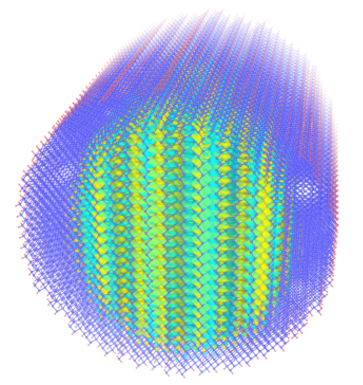
\includegraphics[width=0.3\textwidth]{figs/4-2_2.pdf}
  \caption{カーボンナノワイヤーの電子状態計算}
  \出典{○○○○○(押山淳(東大))}
  \label{fig:4-2_2}
\end{figure}

O($N^3$)の第一原理計算に関しては、実空間密度汎関数法により10万原子の計算が可能であることが示され、実際に大規模手法が開発されている。
また同じく平面波基底の手法でも、金属酸化物材料に対して10万原子規模の計算が視野に入ってきている。
磁性材料や電子相関の強い材料などに関しては、大規模系を扱う場合の収束安定性が課題になると思われるが、この課題が解決するとこれまでの凝集系物理のかなりの問題を直接解明できる。

しかしながら、依然として更に一桁程度多い原子数の取り扱いが必要な問題も残されている。
大規模な計算としては、自己無撞着な計算を一度行うもの、材料に関わるパラメータを変えた複数回の計算から実験的研究結果と比較し得る統計量を抽出するものなどがある。
10万原子を超える計算課題としては、次のような例がある。
(1)半導体金属界面における金属誘起ギャップ状態(MIGS)の存在の有無およびその電気特性への影響。
(2)量子ドットによる新規デバイスの評価・特性予測。
(3)相転移の核形成の問題。
(4)合金における組成の微妙な違いによる塑性変形特性や、弾性特性の変化の予測。
(5)固液界面の問題。

O($N^3$)の手法では、原子数の規模は数万原子程度までで統計量を抽出する需要や反応経路探索などの需要が多くなるであろう。

\rmproject{光・電子材料}
電気・光学・磁気特性を持った機能性材料は、エレクトロニクス、フォトニクス、スピントロニクス等のデバイスを構築する必須要素である。
従来の機能性材料の主役は、シリコン等の半導体に代表される無機物質であるが、近年、その機能性の向上に不可欠な微細加工におけるさまざまな限界が明らかになってきた。
一方、有機化合物や遷移元素を含む有機・無機複合分子を基本とする機能性材料は、その構造および電子的な柔軟さと多彩な分子集合様式に起因するはるかに高い機能性と化学的・物理的制御可能性を備えており、無機材料を凌駕する次世代分子デバイスの基本要素として注目されている。
これらの物質の機能発現機構解明やその合理的設計のためには、個々の分子からその集合相に至る構造・物性・反応の統一的な予測を可能にする高精度かつ大規模な最先端理論計算化学の方法の開発と実行が必須である。

近年、個々の分子やその集合相の相関量子状態において、「電子相関が新機能性発現の鍵となる」という新しい概念が化学と物理の学際領域において見いだされつつある。
また、上述したように、電気・光学・磁気特性単独の機能性だけではなく、今後は電子と光が露わに結合したような状態に起因する電子・光新規機能性次世代ナノデバイスの開発が盛んに行われると考えられる。
具体的な例としては、広帯域・高効率光エネルギー変換デバイス、量子データ転送素子、電子回路に替わり得るフォトニックナノ回路、波長変換素子、メタマテリアル等、きわめて重要かつ新規な機能性を備えた次世代デバイスが挙げられる。これらの高い光・電子機能性を持ったナノデバイスの理論設計を実現するためには、電子ダイナミクスとミクロスコピックな電磁場ダイナミクスが結合した状態を記述するナノ光学理論とその理論に基づく超並列電子・電磁場ダイナミクス法[\要求性能参照{電子電磁場}]の開発が必須である。

\rmproject{生体分子機能・創薬}
近年の急速な構造生物学研究の進展により、膨大な数のタンパク質立体構造の決定が進んだ一方、構造決定が本質的に難しく未解明のものも多数残されている。
この中には、本質的に特定の立体構造を取りにくい、いわゆる天然変性タンパク質や、機能のうえでは複合体を形成して作用するものの、複合体を構造生物学的に安定状態として測定することが難しい過渡的複合体などが含まれる。
このような柔軟性が高く、離合集散して機能する生体分子の原子分子レベルの機能解析が待たれる。
またタンパク質-リガンド間相互作用については、タンパク質の3次元構造は実験によるところが大きいものの、より高い解像度の情報を得るためにQM計算(QM/MM法、フラグメント分子軌道(FMO)法[\要求性能参照{FMO}]、分割統治(DC)法)レベルでの構造最適化が求められている。
また、拡張アンサンブルMD法[\要求性能参照{化学反応動力学}]などによって、タンパク質がリガンドと結合するプロセスを明らかにできるものと期待される。
こうした中間状態の情報は、新しいタイプの阻害剤設計への重要な知見となる。更にはタンパク質分子に加えて脂質も結合した巨大複合体であるHIVやインフルエンザウイルスなど病原性の高いウイルスについて、細胞との結合・解離といった機能の分子レベルでの解明とともに、ウイルス性疾患の予防・治療薬開発への展開も期待される。
このようなタンパク質複合体の構造形成においては、溶媒や塩の効果もきわめて重要であること、更にはタンパク質と脂質膜との相互作用について未解決であることから、全原子の分子シミュレーション[\要求性能参照{長距離古典MD}]による生体機能の分子レベルでの解明が求められている。(図\ref{fig:4-2_3})

\begin{figure}[H]
  \centering
  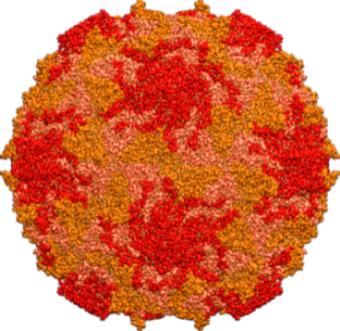
\includegraphics[width=0.3\textwidth]{figs/4-2_3.pdf}
  \caption{ウイルスの全原子計算}
  \出典{○○○○(岡崎進(名大))}
  \label{fig:4-2_3}
\end{figure}


\rmproject{分子構造・分子機能の非経験的予測}
新たな理論と計算方法の開発および計算機の発達とともに、分子構造や分子機能を非経験的に計算から解析・予測できるようになり、計算化学者のみならず実験化学者も量子化学計算を行うようになっている。
今後は、さまざまな分子の基底状態のみならず励起状態を分光学的精度で取り扱うため、相対論、露わに相関した電子状態理論、多参照理論などによる高精度計算[\要求性能参照{高精度分子軌道法}]がより一層重要になると考えられる。

また、FMO法[\要求性能参照{FMO}]やDC法、ONIOM法、電子状態計算と古典力場計算を組み合わせたQM/MM法、3D-RISMやMC-MOZなどの液体論、およびこれを組み合わせた3D-RISM-SCF法などは、巨大分子や溶液系など大規模系の計算を可能にした。
これらにより、実在系の化学反応過程を理解し制御することで、新しい物質変換の開発ができ、創薬、触媒や電池の分子レベルの設計につながると期待される。

更に、上記の領域分割手法に加え、金属などの非局在系を扱うため線形スケーリング手法による全系計算を実現し、ナノスケールで初めて得られる弱い相互作用や立体障害を効果的に利用した機能や構造の提案を目指す。


\rmproject{ソフト分子集団機能}
界面活性剤や脂質・高分子などの多官能性の分子は、温度や塩・共溶媒濃度のような外部パラメータによって、ミセル・膜・液晶といった多様なソフト構造体に自己組織化し、分子の認識、分配、分離、輸送の機能を発揮する。
イオン液体や超臨界流体は、溶媒条件選択による物理的・化学的性質のチューニング幅が大きく、特異的な反応選択性や溶解性・電気特性を発現する。
更に、水のような「通常」の分子集団も、制限空間やクラスレート内では、分子間相互作用を原子レベルで反映して、構造や動的性質を大きく変える。
一般的な高分子材料も、分子配向を高度に制御することにより、従来にない高機能・高強度化を示す。
上記は、規則性とランダム性を兼ね備えた原子・分子集団としての働きであり、ドラッグデリバリーシステム(DDS)、分離膜(海水淡水化等)、食品・コスメティック、生体模倣材料、ガス分離、温暖化ガスの吸収、電池電解液(図\ref{fig:4-2_4})、結晶成長といった広範な学術的・社会的ニーズに直結する。

ソフト分子集団の機能の解析・設計には、原子・分子レベルの相互作用の理解と大域的な集団形状の記述の両方が必要である。
数桁に及ぶ空間・時間スケールの解析には、量子化学計算[\要求性能参照{大規模分子軌道法}]・分子シミュレーション[\要求性能参照{長距離古典MD}]・粗視化シミュレーション・連続体モデルを融合したマルチスケール手法[\要求性能参照{マルチスケール}]の開発が必須である。
特に、実地応用につなげるためには、熱エネルギー程度の分子間相互作用の効果を精度よく取り扱い、化学的個性を取り入れる必要がある。
量子化学計算と分子シミュレーションの大規模化に加え、自由エネルギーを中核とする統計力学理論やレアイベント探索アルゴリズムの高度化が必要である。

\begin{figure}[H]
  \centering
  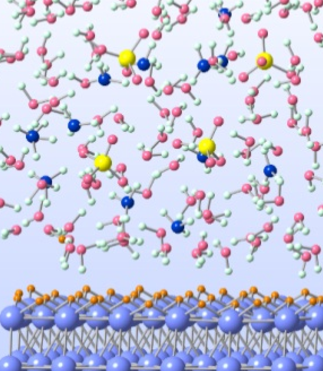
\includegraphics[width=0.3\textwidth]{figs/4-2_4.pdf}
  \caption{電極・電界液界面の第一原理計算}
  \出典{○○○○(杉野修(東大))}
  \label{fig:4-2_4}
\end{figure}

\rmproject{物質・エネルギー変換}
必要な物質を汎用元素から効率よく合成する物質変換法の開発は、わが国の産業基盤の強化に止まらず、地球規模での持続可能な社会を構築するために不可欠である。
このためには複雑な化学反応の微視的理解と予測・制御が必要であり、自由エネルギー面での理論・計算化学研究の遂行が不可欠である。
研究対象としては、複雑な構造を持つ新しい有機分子触媒、金属微粒子、担持触媒、金属表面、金属酸化物表面、金属錯体などが挙げられ、周囲の溶媒などについては数千原子を含めた実際の物質変換系について、1000原子程度の主要部分は量子化学計算[\要求性能参照{大規模分子軌道法}]、周囲は分子力場計算によるQM/MM-MD計算を実行するといったアプローチがある。

また、世界的なエネルギー需要の急増にともない、低コスト・低環境負荷の新規エネルギー変換デバイスの開発が急務になっている。
太陽電池・人工光合成素子の開発では、光吸収過程、電子/正孔キャリアーのダイナミクスの理解と予測、燃料電池、リチウムイオン2次電池などの開発ではイオン伝導、電極と電解質界面での電気化学反応の理解が必要である。
熱電変換素子の開発では、電気伝導度に対する熱伝導度の比率を極力下げる必要がある。
これらすべてに共通する課題は、デバイス全体を構成する複合材料の有するサブミクロンオーダーの巨視的構造とエネルギー変換効率との相関の理解、使用される材料性能の劣化機構の解明と予測である。

これらの課題に対応するためには、有機・無機材料の大規模第一原理計算[\要求性能参照{第一原理}]が必要不可欠である。


\rmproject{界面・表面}
不均一触媒の反応場は典型的な気相・固相ナノ界面であり、半無限の周期性と乱雑さを併せ持つ固体表面と、反応に関わる分子群・微粒子の局所的電子相互作用を第一原理に基づきシミュレート[\要求性能参照{第一原理},\要求性能参照{大規模分子軌道法}]することが可能となってはじめて、理論計算が実験を先導する時代が到来する。
気相表面反応における周期性+乱雑さ+局所性を再現するには少なくとも100ナノメートル四方の領域を露わに扱う必要がある。

気液界面は、大気環境科学との境界領域として、近年特に重要な課題として位置づけられている。工学分野における気液二相流の制御にとっても本質的であり、マイクロバブルなど特異な反応場としての応用も期待されている。

また、固液界面では、固体側の親水性/疎水性を原子レベルで微細制御することが可能になってきている。
界面構造にナノレベルでの凹凸を付けたり、親水性・疎水性の分子を自在に並べるなど、ナノテクノロジーの新たな展開が計算・実験の協業で行われつつある。
また、液体側についても、多成分水溶液系はもちろんのこと、摩擦低減などに使用する炭化水素系の分子など、さまざまな工学応用を目指した物質についての網羅的計算が必要である。

今後、多成分系を含めた実在の界面の解明のためには、界面構造の動的なゆらぎや電気二重層構造のイオン分布を分子シミュレーション[\要求性能参照{短距離古典MD},\要求性能参照{長距離古典MD}]で扱ったうえでマクロな理論につなげる必要がある。

従来の空間・時間スケールを超えたシミュレーションが新展開を示すと期待される。


\rmproject{構造材料の構造と特性の高精度予測・設計}
高精度自由エネルギー計算、第一原理計算、フェーズフィールド法[\要求性能参照{フェーズフィールド}]などを連成したマルチスケール計算[\要求性能参照{マルチスケール}]により、結晶相・化合物相、粒界・界面・欠陥の安定性・強度特性を第一原理から予測し、強度や耐久性、耐熱性を併せ持つ材料や軽量高強度の材料の開発を目指す。

これらのシミュレーションには、典型的にはアレイジョブ、すなわちパラメータを変えた互いに独立で比較的小~中規模のジョブを複数(数十~数万)実行することが必要となる。
小規模ジョブは1ノードで実行され、ノード間通信を必要としない。
中規模ジョブは数ノード~100ノード、大きくても数百ノードで実行される。
1EFlops級の計算機を用いることにより、数千~数万ジョブ規模の計算結果を一度で得ることができる。
アレイジョブの結果からマクロな物理量を取り出し、次の計算へ素早くフィードバックするためにも、アレイジョブが一度に終了することは非常に重要である。


\rmproject{熱交換デバイスの安全性向上・特性解析}
火力、原子力発電所やボイラーなどの熱交換デバイスでは気相と液相が混在する、いわゆる気液混相流(気液二相流)が重要な役割を果たす。
一般に気液混相流は相転移と流動運動がカップルした典型的なマルチフィジックス・マルチスケールな現象であり、マクロな流れとミクロな相転移のスケールの乖離、および相転移をともなうことによる相境界の生成・消滅・移動が数値計算の障害となってきた。

この問題に対しては、これまでは現象をスケールに分け、それぞれの階層において現象論的な支配方程式を仮定することで全体の性質を調べる階層的アプローチが取られてきたが、この方法では各階層のモデル化に任意性が入る上、階層間の接続に経験的なパラメータが必要であった。

一方、気液混相流を構成するすべての粒子(分子)を陽に扱えば、ミクロな粒子間相互作用からマクロな現象を任意性なく再現、解析することが可能となる。
エクサスケールではおよそ100兆粒子程度の自由度を持つ系の計算[\要求性能参照{短距離古典MD}]が可能と見込まれており、実験と直接対応可能なメソスケールに達する。
この、気液混相流の全粒子計算により、より安全かつより高効率な熱交換デバイスの非経験的な設計・開発を目指す。


\rmproject{強相関電子系(超伝導体、磁性体)の機能解明、新物質デザイン}
強相関量子多体系は新しい現象と概念の宝庫である。
実際、高温超伝導、高効率熱電素子、マルチフェロイクスなど近年見出された新物質群の多くが、電子相関の大きな系に属し、その新機能発現機構の解明は、次世代の応用や産業基盤開拓の基礎として期待される。
また、近年実験技術の進歩の目覚しい光格子中の冷却原子系においては、ボーズ・アインシュタイン凝縮をはじめ、ボーズ系モット転移、多種原子系における対超流動、双極子相互作用系での超流動固体状態など、固体中での実証の難しかった量子多体現象が次々に検証されており、更に理論予測を超え、概念の革新につながる系の設計も提案されつつある。

摂動論や平均場近似が破綻するような強相関系では、厳密対角化[\要求性能参照{厳密対角化}]や量子モンテカルロ法[\要求性能参照{クラスター量子MC}]などの量子ゆらぎの効果を正しく取り込んだ第一原理的手法が不可欠である。エクサスケールでは、厳密対角化で50格子点以上、クラスターアルゴリズム量子モンテカルロ法では10億格子点以上のシミュレーションが可能となる。
種々の量子スピン模型、低次元系理論模型のランダムネスの効果も含めた大規模シミュレーションを実行し、物性物理と統計力学の教科書を書き換えるような新概念の数値検証、提案を目指し、物理学の基礎理論の発展に寄与する。

また、第一原理ダウンフォールディング法により、数千バンド、単位胞当たり数百原子以上を含む系の有効模型を第一原理的に導出したうえで、量子モンテカルロ法(数万格子点)、変分モンテカルロ法(数千格子点)[\要求性能参照{変分MC}]などのアルゴリズムを用いたシミュレーションにより、新機能を持った強相関物質材料の物性を高い精度で予測・解明し、材料開発や新デバイス開発を加速する。


\subsection{課題を解決するために必要なアプリーケション群(要求性能)}
\label{sec:4-2_要求性能}
計算物質科学で使われるアプリケーションは非常に多岐にわたる。
以下、計算物質科学分野における、現在の主要なアプリケーション・アルゴリズムの中から、凝縮系に対する第一原理計算、高精度分子軌道法、大規模分子軌道法、フラグメント分子軌道法、電子・電磁場ダイナミクス法、短距離力古典分子動力学法、長距離力分子動力学法、化学反応動力学法、量子分子動力学法、クラスターアルゴリズム量子モンテカルロ法、変分モンテカルロ法、厳密対角化、階層的マルチスケールシミュレーションについてとりあげ、その概略・特性と、今後5~10年で必要となる計算機スペックをまとめる。

\rmproject{第一原理計算(凝縮系)}
\label{sec:4-2_要求性能_第一原理}
半導体材料、磁性材料、光学材料、金属材料などの固体材料を主な計算対象として発展してきた手法が密度汎関数理論(Density Functional Theory(DFT))に則った第一原理計算手法であり、第一原理分子動力学法やバンド計算法という名前で呼ばれることもある。
Kohn-Sham方程式(一電子シュレディンガー方程式)と、電荷密度分布が自己無撞着場(Self-consistent Field=SCF)を満たすように、波動関数と電荷密度分布を繰り返し更新することで解くこの手法の計算需要は、より大きな系の電子構造を精度よく求めるということの他に、長時間の分子動力学計算や統計的処理を行うことにより反応経路や自由エネルギー差などを評価するという、二つの方向に広がりつつある。前者は大規模化を追求する方向性でweak scaling的である。
後者にはstrong scalingを追求するものと、時間やレプリカなど別の軸に関する並列化により計算機能力の向上を有効利用しようとするものとがある。また、励起状態、光学特性、電気伝導特性などの物性予測を高精度に行いたいという需要も大きい。

\subparagraphl{・O($N^3$)法}
扱う原子数$N$に対して演算量が$N^3$に比例する計算方法をO($N^3$)法、$N$に比例する計算方法をO($N$)法(オーダーN法)と呼ぶ。
伝統的なO($N^3$)法の場合、波動関数$\Psi$ を表現する$M$個の基底関数による$M$行$M$列のハミルトニアン行列を対角化して固有値を得るために$M^3$に比例する計算量が必要になるが、CarとParrinelloの提案した方法とそこから発展した方法では、SCFの繰り返しの中で反復解法を使ってより少ない演算数で固有値問題を解くことができる。
基底関数の選び方には、結晶の周期性を利用した平面波を用いるもの、実空間格子点上の値を用いるものなどがある。
全電子ではなく価電子だけを陽に扱う擬ポテンシャル法が大規模計算に適している。価電子軌道の数を$B$とすると演算数は$B^2M$に比例する。
典型的には、$B$は原子数$N$の数倍程度、$M$は100倍程度の値であり、O($N^3$)ではあるが$M^3$の演算数に比較すればずっと少ない。
ここでは擬ポテンシャル法第一原理計算の中で、平面波基底を用いるプログラムとして、PHASEとxTAPPを、実空間基底を用いるプログラムとしてRSDFTを挙げて解析する。
平面波基底は古典的基底でありFFTを頻繁に使うが、原子位置に対して計算精度が不変、行列要素を厳密に計算するのが容易である。
一方、実空間基底は、力の計算精度を上げるのに工夫がいるが、非局所ポテンシャルと波動関数の積の計算負荷が軽いこと、FFT演算を含まないことなどから大規模化に適しているとされる。
また周期境界条件に縛られないO($N$)法への展開が見込める。
平面波基底を使う手法で大規模計算を行うためにはFFT演算にともなう通信を極力局所化する必要がある。
基底関数が何であれ、一回のSCFループ内の計算は、(i)グラムシュミット法などにより規格直交化する部分、(ii)波動関数を残差関数を使って更新する部分(残差最小化法(RMM)、共役勾配法(CG)、Block-Davidson法、最急下降法(SD)など)、(iii)部分対角化する(波動関数のユニタリー変換を行う)部分、(iv)波動関数から電荷密度分布をつくる部分、などからなる。

平面波基底の場合には、負荷の重い部分は、各種の行列・行列積O($B^2M$)と固有値問題O($B^3$)、FFT演算O($BM\log M$)などに分解することができる。
扱う原子数が多くなるに従いFFT演算部分の負荷は相対的に小さくなる。
波動関数に関する3次元FFTはバンド(軌道関数)とFFTの1軸分あるいは2軸分を併せて分割することで、核心部のバタフライ演算はノード内(キャッシュ内)に閉じ込めて行い性能劣化を抑えることができる。
ただし、分割軸を交換するために局所的な転置転送通信を行う必要がある。
非局所ポテンシャルと波動関数の積はO($B^2M$)であるが、並列化効率の向上は容易である。
これに対し(iii)の部分対角化で使うO($B^3$)の固有値問題はそれが難しい。
大規模化するためにはこの部分の効率向上が必要であり、数値計算ライブラリの整備に期待する。
また、波動関数の規格直交化に用いるグラムシュミット法はスレッド並列版のBLASを用いて実装しているが、逐次実行部分が残っている。
これが並列化効率の制限因子の一つとなっている。これに代わる手法の開発も必要である(TSQR法(AllReduce QR法)やCar-Parrinello法を改良した波動関数の規格直交化に用いるグラムシュミット法はスレッド並列版のBLASを用いて実装しているが、逐次実行部分が残っている。これが並列化効率の制限因子の一つとなっている)。

実空間基底を用いる方法は、FFT演算にともなう通信を局所化するなどの手間が要らない、非局所ポテンシャルと波動関数の積演算の負荷が軽いという違いはあるが、(i)規格直交化や(iii)部分対角化に関して抱える課題は、平面波基底を用いる方法と同じである。

O($N^3$)のアプリケーションは、うえで述べたように大規模化と、規模の拡大よりも動的性質を予測するといった方向性の両方を指向するが、ここではRSDFTでは10~100万原子規模の計算を目指し、平面波基底の手法は1万原子規模の系の動的性質を予測する方向を目指すものとして評価を行う。

\subparagraphl{・O($N$)法}
より規模の大きい計算をするために複数のオーダーN法が開発されている。Kohn-Sham方程式の代わりに密度行列を用いる密度行列最適化手法、運動エネルギーを直接電子状態の汎関数で表すOrbital Free DFT法、Wannier軌道のような局在軌道を求める軌道最適化法(Orbital Minimization法)、分割統治法(フラグメント分子軌道法もその一手法)などがある。
オーダーN法に関しては、現状ではさまざまな手法が持つ問題点や計算精度が完全に明らかになっておらず適用範囲が限定的であるが、これらの問題が解決され、いったん標準的な手法になった後は計算時間が原子数に比例するという特性から、特に大規模系に対して標準的に使われる手法になるであろう。
ここでは密度行列最適化によるオーダーN法第一原理計算手法プログラムCONQUESTのエクサスケール計算機に対する要求値などを評価する。
この方法の演算負荷の重い計算には、(i)行列要素計算、(ii)FFT、(iii)局在軌道の実空間座標での値、(iv)疎行列の行列積などがある。
(i)は、密行列の行列積としてBLAS3を複数呼びだす方法を用いている。(ii)に関しては現在Hartree項の計算にFFTを使っている。これは数十万原子までの系では問題とならないが、数百万原子系からは別手法の導入を予定している。
(iii)は基底関数とその展開係数から電荷密度メッシュ(FFTメッシュ)上の値を計算する部分である。
(iv)が最も重い計算であり、通信、行列積演算いずれに関しても、複雑である。通信は隣接通信だけでなく、第4、5近接ノード程度までを含めた近接通信が多い。また疎行列積はパターンの異なる二つの行列の行列積、更に非ゼロの項の一部だけを計算する場合もあるというような特殊な疎行列の積で、非常に複雑である。
またオーダーN性を保つために行列要素の非ゼロ項だけを集めて一次元配列にストアする必要があり、実際の行列要素との対応づけのための複雑なアドレス計算が欠かせない。
更に並列計算では他プロセスから来る隣接原子情報から自分の隣接原子情報への対応表を、演算の前に毎回作成する必要があり、メモリ参照の量に比べて演算数がきわめて少ないという特徴がある。


\paragraphl{【ターゲットとする研究対象】}
計算対象は各種固体材料の他に、固相と液相の界面、固相と気相の界面を含む問題、生体材料などがある。
O($N^3$)法は実空間基底を使うもの(RSDFT)が10万から100万原子規模の材料の電子状態計算を目指すが、100万原子規模の問題を対象とするには現在研究段階の新規アルゴリズムの実用化が必要である。
O($N^3$)法で平面波基底を使うものは1,000から10万原子規模の計算を目指す。O($N$)法は一つの系の原子数は数十万から一億位を目指す。
いずれの手法も、半導体や酸化物のナノ構造、固相・液相界面での安定構造や触媒反応などの反応シミュレーションの他に、バイオ系に対しても第一原理に基づく全原子分子動力学法、更に自由エネルギー計算を行う。
同時に複数個(100~1000個程度)の第一原理計算を行い、拡張アンサンブル法や反応経路計算、自由エネルギー計算などを行うことが重要になる。
この際、O($N$)法では一つの計算が数10万から100万原子、O($N^3$)法では1,000~1万個程度の原子を扱うことを想定している。

\paragraphl{【要求スペック】}

\subparagraphl{・O($N^3$)法実空間基底}
RSDFTで10万原子規模を扱う場合、それがSi原子などである場合、20万程度の固有状態を求める問題となる。
また、格子点は2000万個程度必要である。
対象が金属原子でノルム保存型ポテンシャルを使う場合には、格子点は4億点程度必要になる。
計算主要部分は、共役勾配法、グラムシュミット直交化、部分空間対角化から構成される。
この計算を1日以内で可能な限り短時間で行いたい。
格子点の数をM、固有値数をBとすると、必要なメモリ量は16BM Byteとなる。
10万原子では、60TB~1200TBである。
ノード当たり1TBのメモリがあると想定すれば、問題を乗せるだけで最低でも60~1200ノードが必要になる。
部分空間対角化において$B$×$B$のサイズの行列の固有値問題を解く必要があり、ここでO($B^3$)の演算を行う。
それ以外の箇所は行列行列積の形に還元してBLAS3を呼び出して計算効率を上げることができる。
グラムシュミット規格直交化部分では、演算性能100TFLOPS/node、通信バンド100GB/s、ネットワークレイテンシ1$\mu$sを仮定して、1エクサFLOPS(10,000ノード)のリソースを利用すれば、演算に30秒、通信に21秒要することになる。
通信の大部分はreduction通信である。
部分空間対角化では、$B$×$B$の密行列要素計算にともなうreduction通信、固有ベクトルを求めたあとに各ノードにこれを配るためのbroadcast通信などがある。
行列対角化に要する時間の他に、演算に40秒、通信に74秒が必要である。

\subparagraphl{・O($N^3$)法平面波基底}
xTAPP、PHASEは、波動関数を更新するソルバーの種類、グラムシュミット規格直交化を行うかどうか、3次元FFTの分割方法、並列化軸の設定などの違いはあるが、スペック要求はほぼ同じになるので、まとめて記述する。
10,000原子系の価電子バンド(固有値)の数Bを5×$10^4$、非局所ポテンシャルのプロジェクタの数Pも5×$10^4$、基底平面波関数の数Mを2×$10^6$であると想定する。また、FFTの格子点の数を500×500×500とする。
すると、波動関数用の必要メモリサイズは、平面波係数を倍精度複素数で持つとすると、5×$10^4$×2×$10^6$×16=約1.5TB、局所ポテンシャルと電荷密度用には約2GBである。

ノード当たりの演算性能を10TFlopsとし、一つの構造(レプリカと呼ぶことにする)の計算を1000ノードで行う(1レプリカの計算を10PFlopsで行う)ものとして考える。
また、オンチップメモリはFFTの2次元分の計算ができるだけの大きさ(4MB以上)があるとする。
ネットワークは、リンク当たり50GB/s、トポロジーは10×10×10 nodesの3D meshを想定する(Bisection BWは効率50\%として、2TB/sとなる)。
このシステムでレプリカ1個を担当し、これが100~1,000個並列で動くことで、全体で1~10EFLOPSの計算機能力を使う。
また、レプリカ相互はSCF 1回、あるいはMD計算1回に1度程度通信するものとする。

また、バンドと平面波基底係数の両方を並列化軸にとるのが、規格直交化をグラムシュミット法で行う場合には有利であり、PHASEでは、並列ノード数が1,000の場合にはバンドに関する分割を4、平面波基底係数に関する分割(G分割)を250というように割り当てる。
すると、FFTにともなう通信は、250分割された(G空間上では半径Gmaxの球内に分布している)平面波展開係数を同じく(一つの軸に関して)250分割された(立方体状に分布する)FFT格子点に展開するための転置転送と、FFTの分割軸を変更するための転置転送である。
2次元分のFFT演算は一つのノード内に閉じて行うことにする。
バンド分割だけしている場合には、FFTにともなう通信は必要なくなる。
分割の仕方に関係なくいずれの場合にも、ノード内当たり、500×500の要素の2次元FFTを25,000回、一次元FFTを1.25×$10^7$回行うことになる。
通信時間を無視して、メモリバンド幅を1TBとすると、全バンドのFFTを完遂するのに3秒要する。
しかし、バンド幅が10分の1になると(B/F値=0.01)、30秒程度要することになり、全体の計算時間を圧迫することになる。

行列行列積の大きなものは、非局所擬ポテンシャル(VNL)と波動関数($\Psi$)の積の計算である。
P行G列の行列とG行B列の行列をかけてP行B列の行列をつくり、これにP行G列の行列をかけB行G列の行列をつくる。
前半の積の演算数は2PBG=$10^{16}$になり、10PFlops構成では、計算時間は1秒である。
後半の積の演算は2回行うので計算時間は2秒である。
P、B、Gそれぞれが分割されているとすると、G方向のreduction、B(P)方向のbroadcastあるいはallgather通信が必要になる。
バンド分割が4の場合、前半部分で5GBytesのデータのreductionを行う。
これは50GByte/sの転送能力があれば、隣接ノードに送るのに0.1秒かかる。
全体ではG分割数に応じた通信ステップ数に比例した時間がかかる。
また、B(P)方向のbroadcastは各ノードが持つB/4×G/250×16Bytes=約1.5GBytesのデータを送る。
部分空間対角化にともなう行列要素の作成と、対角化した固有値・固有ベクトルを使って波動関数のユニタリー変換するのにも、同様の行列積計算を行う。

\subparagraph{【計算時間】}
PHASEを使って12,288原子を京速計算機の12,288ノード(×8コア)で計算したとき1SCF(ただし修正最急下降法で部分空間対角化を含まない)当たりの計算時間が約190秒であった(ただし効率は25%弱)ので、これから類推すると10PFlopsクラスターでは1SCFに30秒程度かかることになる。
他のソルバーを使う場合や部分空間対角化法を使う場合には、60秒から100秒程度要すると予測される。
10,000原子に対して、xTAPPのプログラム解析から予測した値、66秒から127秒とほぼ一致している。
1MD計算に20SCF必要であるならば、1MD計算に1300秒から2500秒必要になる。

ここまでノード当たりの10TFlopsの計算能力があるとしてきたが、ノード当たり100TFlopsの能力がある場合には、1構造を100ノードで計算することになる。
ノード数の変化により、bisection B/Wやreductionに必要な段数などが変わり、計算時間は最大15\%程度減少する。

\subparagraph{【メモリ】}
全波動関数係数のデータを保持するのに、ノード当たり約1.5GB必要であるが、他に作業用領域がバンド分割の数を掛けた量必要である。
バンド分割数が10であれば、15GB必要になる。
他にB×Bの部分空間行列、局所ポテンシャル、電荷密度分布などの記憶領域が必要である。
ノード当たり10TFlopsの能力を想定すると、全部合わせて少なくともノード当たり50GB~200GB必要である。
ノード当たり100TFlopsの能力を想定すると、ノード当たり150GB~300GBのメモリが必要である。

\subparagraph{【オンチップメモリ】}
2次元FFTが載るのに十分な量としてチップ当たり10MBとする。

\subparagraph{【ストレージおよびI/Oバンド幅】}
10PFlops相当のノード当たり、最低1.5TB。
1エクサ当たり15PB必要である。I/Oに一つの構造の計算時間の5\%以下の時間を与えるとすれば、1000ノード当たり25GB/s程度の速度が必要である。

\subparagraph{【メモリバンド幅】}
ここではB/F値を0.1程度として予測したが、これが0.01の程度になるとFFT演算に要する時間が10倍になり、実行効率を落としてしまう。
また、規格直交化でグラムシュミットの直交化法を使う場合、並列化効率とノード内の効率が背反する傾向があり、特にノード当たりのバンド数が小さい場合(例えば10,000ノードを使う場合)には、この傾向が顕わになる。
更に、電子相関を高精度化するなどの演算を行う場合には、より大きなメモリバンド幅が必要になる。

\subparagraph{【並列ノード数とB/F値、扱う系の大きさの関係】}
ここでは並列ノード数を1,000程度にして考えたが、O($N^3$)計算では並列ノード数を増やせば必要B/F値は大きくなる関係がある。
またこの関係が系の大きさとも相関を持っており、系が大きいほどB/F値は小さくてもよくなる。
例えば、1,000原子程度の大きさの系を10,000ノードで計算することがバンド幅律速になっており計算効率が悪い場合にはノード数を減らして実行すればよい。
この程度の規模の系の長時間MDを行う目的である場合にはノード数を増やしてstrong scalingの効率を向上する必要があるが、他に例えば統計性を重視する場合には時間に変わる別の並列化軸を設定して、1構造当たりのノード数を抑制することができ、計算機をより有効に使うことができる。
Strong scalingの効率を向上するためのチューニング負荷は大きく、1万原子程度の系に対して京速計算機以上の並列ノード数を使って高い実効効率を達成することは困難が大きいと考えられる。


\subparagraphl{・O($N$)法密度行列最適化法}
CONQUESTで扱う行列には、補助密度行列$L_{i\alpha,j\beta}$や、局所軌道間の重なり行列要素$S_{i\alpha,j\beta}$があり、これらの項の積をつくって計算を進める。
ここで、$i$や$j$は原子の、$\alpha$や$\beta$は軌道の指標である。
原子の指標$i$に関して並列化を行う。
行列のサイズは、(全原子の軌道の数($i\alpha$))×(平均の隣接原子数とその軌道の数($j\beta$))となる。
各行列は異なるカットオフ半径を持つ。
行列積$LSL$などは最も大きな行列の一つである。
「京」の試験利用において、約4000ノードで50万原子系の計算を実現している。
現在のサイズ(100万原子より小規模な系)では静電ポテンシャルの計算に使われるFFTの計算時間はほとんど問題にならない。
将来も古典分子動力学で使われる手法の導入などによりこの部分の計算時間は無視できると仮定する。
1億原子系の第一原理計算を行う場合を考える。
10TFLOPSの性能の計算機ノードを10万ノード使って計算するならば、1ノード当たり1000原子を扱うことになる。
局在基底、オーダーN法の計算は精度によって必要なメモリ、計算時間が大きく変わるが、シリコン系で典型的なカットオフ半径、DZP基底関数の場合、現在1ノード128GFLOPSで1ノード当たり100原子程度でMD計算の1ステップに20分程度かかる。

\subparagraph{【計算時間】}
1ノードで扱う原子数が10倍、1ノードの速度が100倍になるとすると、計算時間は1/10になり、2分程度でMD1ステップの計算ができることになる。
ただし、この実行性能はB/F値が下がれば大きく減少する。

\subparagraph{【通信】}
1ノードが扱う原子数が多くなると通信相手のノードがかなり近いものだけになる。
ノード当たり1000原子を扱う場合には、ほとんど隣接ノードとの通信だけになる。
CONQUESTでは、各ノードが持つ行列要素(と隣接原子の情報、インデックス)は、適宜分割し必要なノードに送られる。
一度の通信におけるパケットサイズはユーザによって制御されるが、この時のサイズはレイテンシが問題にならないためにはある程度大きな量であることが望ましい。
一方、受け取った行列要素を用いて行われる演算は一度に行われるために、受け取った行列要素のサイズがキャッシュに載るサイズであると効率的な計算が行える。
送受信はノンブロッキング通信で行われ、通信と演算の時間を重ねることによって時間を短縮することが可能である。

\subparagraph{【メモリ】}
1億原子の場合の最小基底のシリコンの場合を考慮すると、必要行列サイズは、1×108($i$の数)×1000($j$の数)×4(軌道の数$\alpha$)×4(軌道の数$\beta$)×8(bytes) $\cong$ $10^{13}$(bytes) = 10 TBとなる。
密度行列のカットオフ半径の大きさなどが大きくなる可能性があること、軌道の数も原子当たり13くらいにはなる可能性があること、更に同程度の規模の行列が5~10個あることを考えると、この見積り値に500程度を乗する必要があり、結局、5×$10^{15}$ $\cong$ 5PB程度必要になる。
使用するノードが1000個であれば、ノード当たり5TBのメモリが必要である。この他作業領域などを考えると5~10TB必要である。

\subparagraph{【オンチップメモリ】}
計算速度がノード当たり100倍程度になるとして、それに比例して現状必要な量の100倍として200~300MB程度必要である。

\subparagraph{【B/F値】}
現状の「京」のシステムにおいても計算効率を律速する要因の一つとなっているので、0.2を要求値とする。


\rmproject{高精度分子軌道法}
\label{sec:4-2_要求性能_高精度分子軌道法}
分子軌道法は、基本となるHartree-Fock法を出発点とし、摂動法、結合クラスター法、配置間相互作用法などにより電子相関を取り込み、計算精度を系統的に引き上げられるという特徴がある。
行列積、行列対角化、連立一次方程式計算、そして基底関数の軌道角運動量によって演算内容が異なる1電子・2電子積分計算が主な演算で、計算対象分子を分割しない限り、どの方法でも全対全通信を行う必要がある。
電子相関計算では、中間データ量が系の3乗もしくは4乗に比例して増加するため、各ノードに分散させてもノード当たりの必要メモリ量は多くなる。

エクサスケール計算機では、分光学的精度で分子構造や機能を予測することが期待される。
この目標は、露わに相関した結合クラスター法を完全基底関数極限で解くという、超高精度電子状態計算で達成される見込みである。
ここで、電子相関の計算で必要になる4中心2電子分子軌道積分を、3中心1電子分子軌道積分と求積点での分子軌道の値の積から数値求積法により計算する。
多電子積分計算についても同様に数値求積法で行う。
求積法で2電子積分を計算する部分と、それに続く計算部分をまとめることで演算量を減らすとともに、計算負荷およびデータ分散を容易にする。
主要な演算は行列-行列積である。
各ノードに分散されている求積点ごとのデータを集めるため、通信はallreduce、gathervが大半である。
以下、基底関数極限のフラーレン分子(2万基底、100万求積点)の計算、1ノード性能100TFLOPS、全体性能1EFLOPSを想定して見積もりを行う。

\subparagraph{【メモリ】}
2万×100万(160GB)の配列が4つ、更にその他の配列も考慮して1ノード当たり1TBが必要になる。
メモリバンド幅は、(2万×100万)×(2万×2万)の行列積演算では、1度だけメモリからデータが送られると仮定すると40GB/s、余裕を見て100GB/sが望まれる。
一連の操作を波動関数が収束するまで数十回繰り返し行う。

\subparagraph{【オンチップメモリ】}
求積法で計算する3中心1電子積分用として1GB程度は必要になる。

\subparagraph{【通信】}
2万×100万の配列をgathervで集めた後、上記の行列積演算を4回続けて行うので、計算時間の1割で受信を完了させるためにはノード当たり50GB/sのバンド幅が必要になる。

\subparagraph{【ストレージ】}
計算中のデータはすべてメモリに保存するため、出力するファイルは計算結果のみである。
そのサイズは100TB程度であり、0.01TB/sのファイルI/O性能が必要となる。


\rmproject{大規模分子軌道法}
\label{sec:4-2_要求性能_大規模分子軌道法}
Hartree-Fock法、密度汎関数法によるナノスケール分子の計算を行う。
大部分が2電子クーロン反発積分の計算であり、演算自体は複雑であるが比較的少量のデータを何度も利用するといった特徴がある。
Gauss関数の局所性を利用するため、IF文によるカットオフを多用している。
3次元ナノスケール分子(1万原子系、10万基底)計算を想定すると、30TFLOPSマシン1万ノードの場合、計算時間は1回当たり30分である。
安定構造を求めるためには、この計算を数十回繰り返す。

\subparagraph{【メモリ】}
10万×10万(80GB)の配列を、Fock行列、正準化変換、基底重なり、分子軌道、密度行列用に5つ用意するため、1ノード当たり400GB必要になる。
10万×10万の行列積を行うため、密度汎関数計算での数値積分で1原子当たり1万点グリッドを発生させる場合、ノード当たりのFock行列へのアクセスデータ量は、10万×10万×1万(点数/原子)×1万(原子数) / 1万(ノード)×8Byte = 800TBとなる。
カットオフによるデータ量削減(約10\%に削減)を考慮し1分でこのアクセスを完了させるためには、ノード当たりのバンド幅は1.8TB/s必要になる。

\subparagraph{【オンチップメモリ】}
2電子積分計算のため、1コア当たり1MB必要となる。これは、(gg{\textbar}gg)型積分では、15×15×15×15のサイズの配列にデータを蓄え、同等程度の計算用配列も必要になるためである。

\subparagraph{【通信】}
計算1回(30分)あたり、80GB配列をallreduceで集める操作を30回程度行う。
通信時間を全体の5\%にするには、バンド幅30GB/sが必要になる。

\subparagraph{【ストレージ】}
出力するファイルは計算結果のみで、そのサイズは100GB程度である。
ファイルI/O性能は0.0001TB/s程度で十分である。


\rmproject{フラグメント分子軌道法}
\label{sec:4-2_要求性能_FMO}
フラグメント分子軌道(FMO)法は並列処理を駆使し、タンパク質の電子状態を量子論(QM)的に丸ごと計算することが可能な手法の一つである。
FMO計算は実際には、基本のHartree-Fockから高次相関法まで多種の近似がある。
一般に相関計算では、DGEMM等のBLASを使ったテンソル縮約が支配的で、軌道の添字を複数持つ多次元配列の操作となるためにB/Fが高いほうが性能的には有利である。
だたし、タイリングやブロッキング等を適宜導入することで0.1程度までは性能の保持が可能である。
メモリ要求値に関して述べれば、FMO2のダイマーでクラスター展開の計算では、作業配列の総容量はアミノ酸残基の組み合わせと基底関数にもよるが、数十GBには容易に達する。

現時点で、数百残基のタンパク質の PDB 構造をベースにした一点での FMO2 計算はルーチン的に行えるようになってきているが、より実在的なモデリング手法として信頼性を高めるには、水和条件を課したうえで揺らぎを考慮するために分子動力学的に生成された多数の構造サンプルを扱った統計的な算定が望ましい。
また、3体や4体の展開(FMO3、FMO4)を行うことが、精度向上の観点から望ましい。
フラグメントのトリマーやテトラマーの相対計算コストは数的には単純組み合わせよりは少ないが、個々のサイズが大型化するために増加する。
2次摂動で数百残基のタンパクを扱う場合、FMO2に比してFMO3で3~5倍、FMO4では10倍程度である。
サンプル数の設定によるが、FMO4で相関レベルを上げることまで考えれば、現行計算に比して要求される計算コストは数万~十万倍になるため、エクサ計算機で“統計的ジョブ”の高速実行が可能となれば、その科学的な恩恵はきわめて大きくまた本質的なものとなる。

FMO計算は、光応答タンパク質の電子遷移エネルギーの定量的な算定でも使われてきている。
これは、応答部位(クロモフォア)を特定したうえで限定的に励起状態計算を行うものだが、エクサ級の超並列計算資源があれば、タンパク質全体について求めることも可能であろう。
物性値評価としても、2次高調波などの非線形光学応答核磁気共鳴などの磁気応答などもカバーされる。
光合成系(PSC)の電荷分離のモデリングについても、FMO 計算から得られるフラグメント MO を再構成する(FMO-LCMO)などの技法を用いて大域での電子移動度の算定が行えるようになると思われる。
そこでは数千万次元の非疎行列の固有値問題を解く必要がある。

計算機の環境について付言すると、米国の NWChem ですでに活用されている多ノード共有メモリ空間構築と行列積ツール(GA)等が提供されると大規模フラグメントの処理には福音となると思われる。
また併せて、ノード間をまたぐスレッドベースの並列化もサポートされるとコードの発展には有利であろう。
“統計ジョブ”に関連しては、計算結果をダンプする半導体メモリ(SSD)とともにフォルトトレランス機構が考慮されることが望まれる。


\rmproject{電子・電磁場ダイナミクス法}
\label{sec:4-2_要求性能_電子電磁場}
光機能性を持った量子ナノ構造体デバイスを理論的に設計するための、電子・電磁場ダイナミクスの数値計算シミュレーションソフトウェアである。
対象とする系は、1辺十数nmから数十nm程度の実在系ナノ構造体。
原子数は100万原子から200万原子、時間ステップ数は2.5万~5万ステップである。

\subparagraph{【アルゴリズムの説明】}
時間依存Kohn-Sham方程式(方程式の形は時間依存シュレディンガー方程式と同一)を実空間3次元グリッド上で差分法を用いて解く。
x,y,z方向の格子点数を各々Nx,Ny,Nzとすると、実空間グリッドの総数はNx×Ny×Nzとなる。
主要な演算は、ハートリーポテンシャルを評価するためのポアソン方程式の計算、時間発展計算にともなうハミルトニアンの波動関数への作用の二つに大別できる。
いずれにもラプラシアンの作用が含まれており、その演算は、((Nx×Ny×Nz)×(Nx×Ny×Nz))の疎行列と(Nx×Ny×Nz)のベクトルとの積と等価である。
ただし、実際の計算では疎行列そのものを扱うのではなく、縮約してベクトルとベクトルの積に帰着する。
マクスウェル方程式も実空間3次元グリッド上で差分法を用いて解くが、Kohn-Sham方程式に比べればその計算負荷は格段に低いので相対的に無視できる。

\subparagraph{【想定する計算】}
光機能性を持った量子ナノ構造体デバイスを設計するためには、最低50000ステップの時間発展が必要となる。
C60分子を立方体空間に25個×25個×25個~16000個並べる系を想定してスペックを見積もる。
この場合、原子数は60×16000分子~960000個、軌道数は120×16000分子~1.9M軌道となる。

\subparagraph{【想定する計算機】}
時間発展1ステップ当たり1秒で計算を行うためには、630PFLOPSのシステムが必要になる。

\subparagraph{【計算空間総メッシュ数】}
メッシュサイズを0.25Åとすれば1辺当たり33nm÷0.25Å~1300点。
したがって、総メッシュ数は(1300)3~2.2Gとなる。

\subparagraph{【総演算量】}1ステップ当たり2.2G(総メッシュ数)×1.9M(総軌道数)×30回(差分法演算回数)×5回(テーラー展開4次+軌道エネルギー評価)~630P回。

\subparagraph{【総メモリ量】}
計算グリッド上に波動関数をストアしておくためのメモリがほとんどを占める。
2.2G(総メッシュ数)×1.9M(総軌道数)×16B(複素数)×3(作用前波動関数用配列、作用後波動関数用配列、テーラー展開での総和の波動関数用配列)~200PB。

\subparagraph{【ネットワークバンド幅】}
1ステップ当たり2.2G(総メッシュ数)×8B(実数)~18GBの電子密度用データのAllreduceによる通信が発生する。
通信を全実行時間の1割と考えるとノード当たり180GB/s必要となる。

\subparagraph{【メモリバンド幅】}
1ステップ当たりの総メモリ量を1秒でアクセスするために200PB/s必要となる。

\subparagraph{【オンチップメモリ】}
1軌道当たりに必要とされるメモリ量は2.2G(総メッシュ数)×16B(複素数)×3(波動関数用配列数)~110GB。
空間を125分割(5×5×5分割)して、各ブロック内で差分法演算に使うデータをすべてオンチップ上に載せるためには0.9GB必要になる。

\subparagraph{【ストレージ容量】}
波動関数を入力として読み込むために、2.2G(総メッシュ数)×1.9M(総軌道数)×8B(実数)~33PBが最低必要となる。


\rmproject{短距離力古典分子動力学法}
\label{sec:4-2_要求性能_短距離古典MD}
主にカットオフのあるLennard-Jones型ポテンシャルなど、短距離相互作用の粒子モデルを古典分子動力学法により時間発展させ、気液二相流を全粒子計算によりシミュレーション、解析を行うというものを想定する。
この場合、計算コストの大部分は二体力の計算であり、並列化は3次元空間分割、通信は隣接ブロックとの粒子座標交換となる。
なおプロセス全体のフラグ同期を毎ステップともなう。
想定する計算機の性能は、100TFLOPSの計算能力と10TBのメモリを持つノードが全体として1EFLOPSを構成しているとし、この計算機上で粒子数$10^{12}$から$10^{14}$程度、粒子数×ステップで$10^{18}$~$10^{20}$程度の計算行うとして通信およびストレージへの要求性能の見積もりを行う。

\subparagraph{【計算可能な総自由度の見積もり】}
例えばカットオフ3、密度0.5の系を想定すると、粒子当たり50回の力の計算が必要となる。
粒子対当たりの浮動小数点演算回数はおよそ50回であり、力の計算を全体の5割、1ステップを1秒以内で行うことを考えると、100TFLOPS程度の計算能力があれば、20G個程度の粒子の計算が可能となる。
しかし、現在の実装では密度揺らぎのバッファも含めて粒子当たり2KBのメモリを必要とするため、ノード当たり10TBのメモリがあるとすれば5G個の粒子までしか扱うことができない。
このように短距離古典分子動力学法においては、計算が比較的軽いため、扱うことができる粒子数は計算能力よりもメモリ容量によって規定される。
以上のようにノード当たり5G個の粒子を扱い、1万ノードあれば、50T個、すなわち50兆粒子の計算が可能となる。

\subparagraph{【メモリバンド幅】}
理想的にキャッシュ、レジスタが使えた場合、一つの力の計算を行うのに粒子座標の3成分を読み込み、運動量の3成分を書き込む必要があるため、1粒子対当たり48Byteの読み書きが生じる。
1粒子対当たり50演算を行うため、演算器を使い切るためにはB/F値は1.0程度必要となる。
しかし、力の計算を理想的に行った場合でも演算器を半分程度使うのが限度であると思われるため、ピーク性能比として20\%を目指すのであれば、B/F値は0.20程度でよい。

\subparagraph{【通信バンド幅】}
100TFLOPSの計算能力を持つノードに5G個の粒子を載せた場合、粒子直径を1としておよそ2000×2000×2000の領域に対応する。
したがって、通信量は1step当たり2000×2000×3(カットオフ)×6(方向)×24Byte=1.73GB程度となる。
1stepの計算に0.25秒程度かかると推定されるため、通信が0.01秒程度で完了することを要求すると、100GB/sから200GB/s程度必要となる。
ただし、通信と計算を完全にオーバーラップさせることができれば、5GB/sから10GB/s程度でよい。
また、アルゴリズム上、毎ステップすべてのプロセスで同期が必要となるが、1stepが比較的長いため、通信および同期のレイテンシはほとんど問題にならないと思われる。

\subparagraph{【ストレージ】}
物理量は原則として計算中にTBオーダーまで粗視化したうえで出力することを想定している。
そこで、ストレージはチェックポイントファイルがストレスなくはける程度でよい。
50T個の粒子情報をすべて出力すると2.4PB程度となる。
一度のプロダクトランで数回出力するとして10PB程度。
頻繁に保存しないため、数十秒かかってもよく、0.1PB/s程度のI/O速度があればよい。


\rmproject{長距離力古典分子動力学法}
\label{sec:4-2_要求性能_長距離古典MD}
脂質膜や高分子の大域構造やダイナミクス、特に、単純な球や平面を超えた現実的な曲率を持つ系の取り扱い、また、タンパク質複合体の解析には、1億〜10億原子系を対象として、マイクロ秒〜サブミリ秒の計算が必要となる。
ナノ界面の取り扱いにも、原子レベルの凸凹を含めて、固体部分と液体部分の分子を露わに取扱うために、数千万原子系についてマイクロ秒〜ミリ秒の計算が必要となる。

ここで必要な計算スペックを、modylasの「京」でのMD計算のパフォーマンスを基に試算した。
マシンの性能を5 EFLOPSと想定し、単ノード当たり10 TFLOPSであったとすると、ノード数は50万となる。
よって単ノード当たりの原子数は1~10億÷50万=200~2000となる。
「京」ではノード当たり160原子程度が最適であったので、ノード当たりの負荷は約1.2~12倍となる。
メモリについては、MODYLASによる実測に基づき10億原子系について試算した結果より、全ノード合計で2PB程度必要となる。
また「京」と同程度の容量のL1,L2キャッシュが装備され、SIMD機能が備えてあればよい。
更に単ノード当たりの性能は「京」に比べて10T/128G=78倍となっており、これが原子数増大による負荷1.2~12倍および1 MDステップ当たりの処理速度の向上(6~60倍程度)に費やされると考えれば十分に実行可能である。

ノード当たりの通信量は、ノードに含まれる原子数に比例するとして、約1.2~12倍となる。
「京」での数十マイクロ秒の12倍時間を要したとするとサブミリ秒程度である。
目標は1MDステップを0.1~1ミリ秒程度なので、通信速度は「京」よりやや速いものが必要となる。
更に、「京」においてはレイテンシにサブミリ秒を要しているが、高速化のためにはこれを数分の一にする必要がある。

MDのトラジェクトリは、1 psごと程度に保存することが妥当である。この場合に必要な総ストレージ容量は、約100~1000 PBとなる。


\rmproject{化学反応動力学法}
\label{sec:4-2_要求性能_化学反応動力学}
反応経路上に複製された多数のレプリカ構造を等間隔に配置しつつ構造緩和させることで最小エネルギー経路を求めるString法やNudged Elastic Band法、反応経路のアンサンブルを発生するTransition Path Sampling法やOnsager-Machlup法、反応座標を拘束した分子動力学計算から反応自由エネルギー曲線を計算するBlue Moon Ensemble法、バイアスポテンシャルを用いて反応自由エネルギー表面を探索できるMetadynamics法などがある。
また、少数自由度系について網羅的に探索することのできるGRRM法やAFIR法もある。
非断熱遷移をともなう反応にはSurface Hopping分子動力学法などが不可欠である。
更に、分子振動状態を扱うvibrational SCF法などがある。
これらの手法の場合、レプリカを多数(数十~数万)用いた同時並列計算になるが、レプリカ間は座標・エネルギー・力などを交換や収集するだけで、通信量は少なくてすむ。


\rmproject{量子分子動力学法}
\label{sec:4-2_要求性能_量子MD}
経路積分法により虚時間軸上に複製されたレプリカについて分子動力学計算を同時に並列で実行すると、零点振動・トンネル効果など量子現象を考慮した分子シミュレーションが可能になる。
これを更に電子状態計算と組み合わせると、電子と原子核からなる量子多体系を丸ごと第一原理的に解ける。
この方法によれば、水素をはじめとした軽元素の物性の定量的解析が可能となり、水・DNA・酵素など水素結合系の分野で貢献できる。
また、この特徴を活かし、実験とのタイアップのもと、次世代エネルギーとして期待される水素貯蔵材料、燃料電池材料の研究開発に役立てることもできる。

経路積分分子動力学法では、数十~数百レプリカそれぞれについて、延べ数十万~数百万ステップ程度の統計量をとる必要がある。
隣接するレプリカ同士には調和振動子的相互作用が作用するため、各ステップで、座標・エネルギー・力などの通信が発生する。


\rmproject{クラスターアルゴリズム量子モンテカルロ法}
\label{sec:4-2_要求性能_クラスター量子MC}
量子スピン系、ボゾン系などの量子格子多体系において、量子ゆらぎの効果と温度ゆらぎの効果を厳密に取り入れた量子モンテカルロシミューレーションを行うというケースを想定する。
具体的には、連続虚時間経路積分を用いて、量子格子模型を一つ次元の高い古典模型にマップ(世界線表示)して計算を行う。
この手法の特徴は、世界線の更新にループクラスターアルゴリズムを用いる点にある。
すなわち、世界線を局所的に更新するのではなく、ループと呼ばれる大域的な単位(かたまり)で更新する。
ループの生成は、ループのサイズが系の内部自由度の相関とちょうど対応するように、かつ厳密につりあい条件を満たすように構成される。
そのため、マルコフ連鎖の緩和は非常に速く、数百万~数億原子系においても自己相関時間は1~100程度である。
これにより、計算機のメモリをフルに利用するような超大規模系においても、精度の高い平衡状態のシミュレーションが可能となる。

一方で、毎モンテカルロステップにおいて、全系の中でループを認識する必要があり、そのためのunion-findアルゴリズムが計算時間の大部分を占める。
ここでは、リンクリストをたどる、リンクリスト同士を結合する、など非浮動小数点数演算が主であり、ベクトル化やSIMD化は非常に困難である。
CPU単体性能としては、条件分岐やキャッシュミスのペナルティが小さいことが求められる。
すなわち、レイテンシの短い演算器、レイテンシが短くインダイレクトアクセスの速いメモリが必要である。
更に、ノード間ではバタフライ型の通信により、大域的なループ認識処理を行うので、輻輳を抑えるためにも高次元のネットワークが必要となる。


\rmproject{変分モンテカルロ法}
\label{sec:4-2_要求性能_変分MC}
数百~数万原子からなる大規模な強相関電子模型・量子スピン模型の基底状態波動関数を計算するというものである。
多数の変分パラメータを持つ変分波動関数について、エネルギーの期待値をモンテカルロ法で評価し、変分パラメータを最適化することで、基底状態の波動関数・エネルギー・さまざまな物理量の評価を行う。
他の手法では扱うことの難しい2次元以上の強相関電子系やフラストレーションのある量子スピン系を精度よくシミュレートすることが可能である。
例えば「京」では1000格子点規模のシミュレーションにより鉄系超伝導特性の物質依存性が明らかにされつつあるが、これを超える高温超伝導体の設計指針を確立するためには、より高い精度での理論予測の検証や実験系との定量的な直接比較による新機能発現機構の解明が必要である。
そのためのシミュレーションには、多軌道効果や格子歪効果を取り入れた数万格子点規模の計算が必要であり、「京」の100倍程度の計算機環境が必要となる。

変分モンテカルロ法のボトルネックは、変分パラメータの最適化における逆行列の高速更新である。
行列のサイズは電子の数(数千〜数十万)である。
5回=40Byteの読み書きに対して32の演算があるため、B/F値は1.25と見積もることができる。
また、計算条件によっては、行列のパフィアン(行列式の一種)の高速更新における行列ベクトル積(B/F値=8)がホットスポットとなる場合もある。
アプリケーション全体としてのB/F値は1.5程度と見積もられる。
ノード数10000、1ノードの理論ピーク性能100TFLOPS、合計で1EFLOPSの計算機を想定すると、20\%の実効性能を実現するためにはメモリB/F値=0.3が必要となる。
ノード当たりのメモリ容量は1TByte、ネットワークバンド幅とディスク容量については「京」と同程度で十分である。

以上の性能を持つ計算機を1ヶ月程度専有することで、上記の目的を達成することができると考えられる。


\rmproject{厳密対角化}
\label{sec:4-2_要求性能_厳密対角化}
量子スピンが相互作用する多体系のハミルトニアン行列をランチョス法により対角化することを想定する。
量子多体系のハミルトニアン行列は、疎行列であるが、非零要素が対角要素から遠く離れたところにも多く表れるのが特徴である。
計算コストの大きな箇所は、行列を巨大ベクトルに作用させる部分で、計算は、この演算の繰り返しとなる。
行列要素はon the flyで計算する。
行列作用の回数は、バタフライ型の転送を要する行列と転送なしのケースがあり、総回数は10万~100万回。
巨大ベクトルの次元に比例する時間とメモリ(分散メモリの合計でよい)が必要である。
以下、ノード当たりメモリ量、バイセクションネットワークバンド幅としては比較的高い値を持つハードウェア、具体的には、1ノード性能として5TFLOPS (整数演算も同じ性能と仮定)・5TBメインメモリ・512MBオンチップメモリ、総ノード数$2^{14}$=16384、全体性能として82PFLOPS・メモリ82PB、バイセクションハンド幅2PB/s (High-radix型のトポロジーを仮定)のハードウェアを想定し、性能の見積もりを行う。

\subparagraph{【計算する物理系と計算規模】}
1次元のS=1/2スピン系を考える。
スピン(格子点)数は54とする。
このとき、行列・ベクトルの次元は${}_{54}\mathrm{C}_{27}$=1,946,939,425,648,112、1ノードのメモリ使用量最大値(40スピン分)=${}_{40}\mathrm{C}_{20}$(要素)×8(B/要素)×5(本)=5,513,861,152,800B=5TB、総メモリ使用量=${}_{54}\mathrm{C}_{27}$(要素)×8(B/要素)×5(本)=77,877,577,025,924,480B=69PBとなる。
この超巨大規模の行列・ベクトル積演算を一回当たり100秒程度で行うことを想定する。

以下では、キャッシュ(オンチップメモリ)上にロードしたデータを最大限に利用するため、ベクトルを(最大)${}_{26}\mathrm{C}_{13}$=9.9M要素(79MB)単位でブロック化してメインメモリからオンチップメモリにロードするものとする。
ブロック数は$2^{14}$=16Kとなる。
また、インデックスの逆引き用分割テーブル(少し大きい)と局所ハミルトニアンの行列要素のテーブル(非常に小さい)は計算の最初から最後まで常にオンチップメモリ上にあるとする。

\subparagraph{【1ノード内での演算量・メモリ転送量】}
対角ブロック部分は計16K個のブロックからなる、各ブロックは9.9M要素の対角成分と、25×9.9M要素の非対角成分からなる。
対角成分の乗算にはインデックス計算は必要ないが、行列要素の計算には、1要素当たり、局所ハミルトニアン行列のインデックス計算に5整数演算(shift×2+and×2+or×1)、その和に1浮動少数点数演算が25セット必要である。
ベクトルの要素との乗算には2浮動少数点数演算が必要となる。
また、非対角成分の乗算には、1要素当たり、ベクトルのインデックス計算(6整数演算)、局所ハミルトニアン行列のインデックス計算(5整数演算)、ベクトルの要素との乗算(2浮動少数点数演算)が必要となる。

一方、非対角ブロックは、合計で14×16K個あるが、非対角ブロックの非零要素(9.9M個)はすべて非対角成分である。1要素当たり、ベクトルのインデックス計算(6整数演算)、局所ハミルトニアン行列のインデックス計算(5整数演算)、ベクトルの要素との乗算(2浮動少数点数演算)が必要となる。

以上を合計すると、ノード内非並列部分合計として、1回ハミルトニアンを掛けるのに必要な演算数は、浮動小数点数演算=((1×24+2)×9.9M+2×24×9.9M+2×20×9.9M)×16K=181,00G=17.6T、整数演算数=(5×24×9.9M+(6+5)×24×9.9M+(6+5)×20×9.9M)×16K=95,700G=93.4Tとなる。
一方、メインメモリアクセスは、左辺ベクトルのload/storeが79MB×16K×2、右辺が79MB×(1+20)×16K、合計29,100G=28.4TB必要である。
したがって、ピーク性能を出すために必要なB/F値=28.4/17.6=1.61(もしくはB/(F+I)値=0.256)と見積もられる。

\subparagraph{【並列部分】}
1回のハミルトニアン乗算に以下の転送演算が16回必要となる。
転送パターンはバタフライ型である。
ノード当たり転送量は1TB×2のsend/receive、すなわちバイセクション転送量は1TB×16384=16PBとなり、一回の転送に8秒かかる計算になる。
演算に関しては、インデックス計算・行列要素計算はほぼ無視できる一方、浮動小数点数演算数は2×0.125T=0.25Tであるので、0.05秒で完了、また、メインメモリへのアクセス量は3×1TB=3TBであるので、0.6秒で完了する。
以上の見積もりから、律速となるのはノード間転送であることがわかる。
すなわち演算とメインメモリアクセスはすべて転送の裏に隠せることになる。
ノード間計算部分では「バイセクションバンド幅」が計算の律速となる。

\subparagraph{【全体性能】}
全計算時間は((17.6+93.4)/5+8×16)×1000iteration=150,200sec=42hourと見積もられる。
このうちノード間転送時間が全体の85.2\%を占める。
仮にバイセクションバンド幅が10倍になると全計算時間は9.7hourまで短縮される。
逆に1iterationを100sec(すなわち全計算時間を106sec)以内で終わらせるためには、3.3PB/sのバイセクションバンド幅が必要となる。

\subparagraph{【ストレージに対する要求】}
最終的な結果の出力はごくわずかであるが、チェックポイント用にベクトル3本(計41PB)分の入出力が必要である。この読み書きを30分程度で終了するI/O性能が要求される。


\rmproject{階層的マルチスケールシミュレーション}
\label{sec:4-2_要求性能_マルチスケール}
階層的マルチスケールシミュレーションとは、二つ以上の異なるプログラムを縦列に接続することにより、個々のプログラムでは得られない物性を引き出す手法である。
具体的には、下部プログラムである第一原理電子状態計算(量子化学計算、バンド計算、FMO計算、ONIOM計算など)や古典力場計算(短距離力、長距離力)あるいはその組み合わせ(QM/MM計算やRISM-SCF計算など)を同時に複数並列で実行し、これに必要な入出力情報(原子核の位置、エネルギー、力、その他の物性情報)を通信で交換または収集する。
次に、上部プログラムである分子シミュレーション法(分子動力学法、モンテカルロ法、拡張アンサンブル法など)や理論(統計力学、線型応答理論、化学反応論、経路積分理論)に基づいて追加的に処理を施す。
以上が基本工程になっている。
そして、目的とする物性データを最適化したり、統計的処理を施したりするのに、この基本工程を大量に繰り返す必要がある。
この際、下部プログラムが全計算の大半を占めるため、計算に必要なスペックは下部プログラムの種類に準じて決まる。
通信は不可欠であるものの、通信量は限られていることから、超並列アーキテクチャをうまく活用できるという特徴があり、化学反応、量子分子動力学、相転移、相図、熱物性、分光学的・電気的物性、材料強度など、広範な応用が期待される。

このシミュレーションでは、上部ソフトウェアと下部ソフトウェアが独立している場合、現状ではシステム・コールとディスクI/Oを介した情報交換を多用せざるを得ない。
これを避けるためには、各ソフトウェアのインターフェースやMPIコミュニケータを著作権に注意しながら適宜書き換える必要が生じる。


\subparagraphl{・クラスター展開法:相図の第一原理計算}
クラスター展開法での相図の第一原理計算では、100~10,000原子のスーパーセルを対象とし、100~1,000の異なるイオン配置について平面波基底の第一原理分子動力学法を同時に並列で実行し、それぞれの安定構造と全エネルギー値を収集する。
次に、これをもとに決定されたイオン間の相互作用から、1,000から10,000のモンテカルロ計算を行い、相図を求める。

エクサスケール計算機の活用により、2元系合金にとどまらず3元系合金の相図を一度の計算で求める等の応用が期待される。
例えばATAT (http://www.brown.edu/Departments/Engineering/ Labs/avdw/atat/) やCLUPAN (http://clupan.sourceforge.net/)が代表的なアプリケーションである。


\subparagraphl{・凍結フォノン法:熱物性の第一原理計算}
凍結フォノン法は、第一原理計算から得られるフォノン分散関係から熱物性を計算する手法である。
比熱評価のためには、約100原子のスーパーセル中の一つのイオンを微小に変位させた多数の構造で平面波基底の第一原理計算を同時に並列で実行し、それぞれで得られた各イオンに働く力を収集して得られるダイナミカル行列を対角化して、フォノン分散関係を求める。

熱伝導率評価のためには、高次の非調和相互作用項の計算が必要であり、そのためにはより大きなスーパーセル(100~10,000原子)を用いてスーパーセル中のイオンを複数個変位させた第一原理計算を同時に実行する必要がある。
例えばphonopy (http://phonopy.sourceforge.net/)が代表的なアプリケーションである。

\subparagraphl{・有効ハミルトニアンに基づいた分子動力学法:強誘電体物性}
強誘電体を擬スピンが格子状に並んだモデルとして考える。
その有効ハミルトニアンは第一原理計算から決定する。
有効ハミルトニアンを温度、圧力、ひずみ、バルクか薄膜か、外部電場などさまざまな環境下で分子動力学法により時間発展させることで強誘電体の物性、すなわち相図やリラクサーの誘電率の周波数依存性などが決定できる。
このためには、256×256×256~512×512×512ほどの3次元FFT(実数→複素数、複素数→実数)を多用する、1ノードに載る比較的小規模の計算を数百~数万個実行する必要がある。
例えばferam(http://loto.sourceforge.net/feram/)が代表的なアプリケーションである。


\rmproject{フェーズフィールド法}
\label{sec:4-2_要求性能_フェーズフィールド}
フェーズフィールド法は、合金材料の組織形成をシミュレートする連続体モデルであり、実用合金の実プロセスにおいて問題となる組織形成過程の解析に応用されつつある手法である。
合金凝固過程を対象とすると、流体の速度場、温度場、溶質拡散場および秩序変数の方程式を連立して解くことになる。
フェーズフィールド法において、デンドライト組織形成を高精度にシミュレートするためには、$10^{-8}$~$10^{-7}$m程度の空間分解能を要する。
一方で、デンドライト集団の統計的挙動の議論において対象とする空間スケールは$10^{-3}$m程度のスケールである。
したがって、凝固組織形成の高精度シミュレーションには、おおよそ1013~1014規模のメッシュ数が必要となる。
並列化による大規模計算における主たる演算は陽解法によるステンシル型の計算であり、袖領域のデータ通信が並列化における通信時間の主となる。
現在、TSUBAME2.0を用いたGPU並列により、$10^{12}$メッシュ規模の計算で2PFlopsの実行性能が達成されている。

ミリメートルの空間スケールにおける数分間の実用合金の一方向凝固を、24時間程度の計算時間でシミュレートするために要する性能を見積もる。
総メッシュ数は$10^{13}$~$10^{14}$程度であり、1万ノード並列を仮定すると、1ノード当たりのメッシュ数は$10^9$程度となる。
また、実時間スケールで数分間のシミュレートのために必要な総時間ステップ数は$10^7$程度であり、一ステップあたり$10^{-2}$s程度の計算時間である。
これに基づくと、1ノードの理論ピーク性能は100TFLOPSが必要となり、全体で1EFLOPSを要する。
そして、この計算に必要な一ノード当たりのメモリは約150GBとなる。
また袖領域の通信容量は一ステップあたり300MBと見積もられ、通信には少なくとも30GB/sが必要となる。

\rmproject{まとめ: 物質科学分野が必要とする計算機環境}
計算物質科学におけるアルゴリズム・シミュレーションの特徴として、以下が挙げられる。

\begin{itemize}
\item 1回の時間発展の計算だけではなく、相関の強い系や平衡状態や定常状態に興味がある。
\item 非平衡状態を議論する場合には、フェムト秒からピコ秒、ナノ秒といった非常に長時間のシミュレーションが要求される。
\item シミュレーションする系の次元は3次元とは限らない。
相関の強い量子多体系のシミュレーションでは、相互作用が非局所的であることも多い。
\item 遠くの相関の効果を正確かつ効率的に取り込む、または、できる限り少ない反復回数で平衡状態にたどりつくためのアルゴリズム上の工夫として、非局所的な操作が導入される場合も多い。
\end{itemize}

このため、局所性が乏しくデータの再利用が困難、物理的に遠くのノードとの通信が必要となり高次元のネットワークトポロジーが必要など、一般的に高い性能を持つハードウェアが要求される。

\paragraphl{【演算器・メモリ】}
計算物質科学分野のアプリケーションが要求する性能は、演算重視、メモリバンド幅重視、クロック重視など、さまざまである。
しかしながら、他の分野と比べ、一般的に大メモリ、高メモリバンド幅を必要とするアルゴリズムが多いと言える。一方で、浮動小数点数演算が少なく、SIMDが全く効かないアプリケーションも存在する。
物質科学分野としては、「京」と同様のアーキテクチャー、あるいはメモリと演算とのバランスをより重視したアーキテークチャを中心とした、複数のシステムが望ましい。

また、物質科学分野においては、非常に短いサイクルで新しい手法・アルゴリズムが次々と生まれているため、分野全体として必要とする演算の種類、B/F値などをあらかじめ想定すること不可能である。
したがって、ヘテロな構成のCPUの場合、ほとんどの場合その性能を使い切ることは困難であると考えられる。

演算精度については、安定性、精度の面から単精度では不十分な場合が多く、通常倍精度演算が必要である。
一方、現状では4倍精度への要求はそれほど強いとは言えない。
しかしながら、エクサスケールの計算機により長時間シミュレーションが可能になってくると、倍精度の限界が見えてくる恐れも十分にある。

\paragraphl{【ネットワーク】}
物質科学分野のアプリケーションにおいては、3次元の隣接通信だけではすまず、4次元あるいはより高次元の通信パターンが必要となる場合も多い。
そのため「京」のような3次元メッシュ/トーラスではネットワークがボトルネックとなり演算性能が発揮できない場合も多い。

エクサスケール機のネットワークとしては、high-radixタイプのものが望ましい。
あるいは、遠くは3次元トーラス、近くはより次元の高い密な結合といったハイブリッドタイプのネットワーク構成と、特にallreduce, allgather, alltoallといった全対全通信を効率よく行うための機構や、FFT、疎行列の対角化、クラスターモンテカルロ法におけるバタフライ型通信・演算のための機構を組み合わせた全く新しいネットワークの開発が求められる。
一方、strong scalingで長(実)時間の計算を行う場合のボトルネックはレイテンシである。
近接通信、あるいはリダクション演算を現状と同程度あるいは現状より更に低いレイテンシで実行可能なネットワークが望まれる。

% 要求性能表
%\clearpage
\input ReqSpecTabs/4-2.tex

\subsection{他分野との連携}
理論物質科学、すなわち理論物性物理、理論分子科学、理論材料科学は、古くから実験分野との強い連携の下に研究が進められてきたのは言うまでもない。
今後は、J-PARC、SPring-8、SACLAといった大型実験施設との、より一層の連携が求められる。
また、物性理論分野は、素粒子、原子核、宇宙といった他の基礎物理分野とも強い関連があり、伝統的に研究交流も盛んである。
近年では、生体分子研究における生命科学分野との連携や、エネルギー・環境分野におけるものづくり分野との連携も進んでいる。


\subsection{公的な意見交換とそのサマリー}
物質科学分野では、討論会「エクサスケールコンピュータへの期待」(2012年7月13日、東大物性研)、日本物理学会計算物質科学インフォーマルミーティング(2012年9月18日、横国大)、TCCI研究会(2012年10月9日、分子研)、計算物質科学シンポジウム(2012年10月22日、東大物性研)、CMSI研究会(2012年12月3日、分子研)、日本化学会特別企画「超巨大計算時代の化学」(2013年3月25日、立命館大)、日本物理学会シンポジウム「エクサスケールに向けて歩み出す計算物理学」において、実験家、企業研究者も含めたコミュニティ全体に対しロードマップを紹介し、パネルディスカッションなどを通じて意見収集を行った。
具体的には、J-PARC、SPring-8、SACLAといった大型実験施設との連携強化、元素戦略(磁石、触媒・電池、電子材料、構造材料分野)への計算物質科学からの貢献への期待などの意見を得ることができた。
また、最先端HPCだけでなく、非専門家がPCあるいはクラスターワークステーションでシミュレーションを実行できるよう計算物質科学コミュニティ全体でアプリケーション・ソフトウェアを整備することや、莫大なシミュレーション結果や実験結果を保存・公開する仕組みを整備することなどに対する強い要望があった。


\subsection{ロードマップ}
\begin{figure}[H]
  \centering
  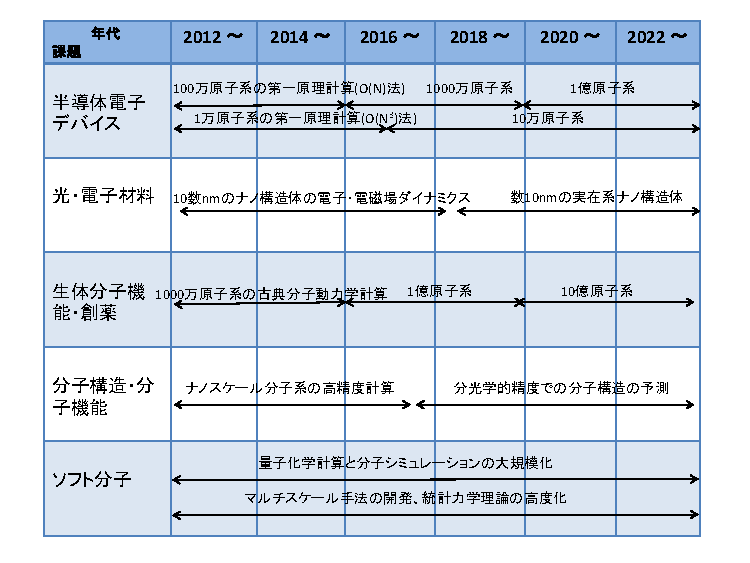
\includegraphics[width=0.7\textwidth]{figs/4-2_rm_1.pdf}
  \caption{物質科学ロードマップ(1)}
  \label{fig:roadmap_4-2_1}
\end{figure}
\begin{figure}[H]
  \centering
  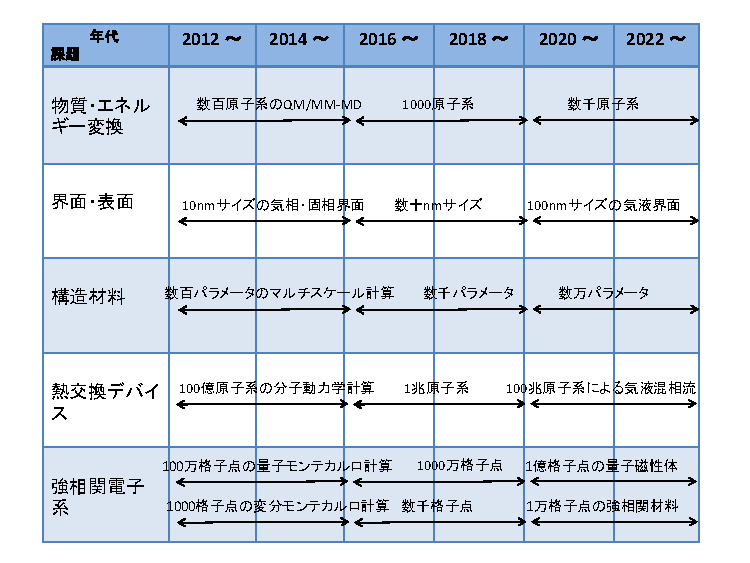
\includegraphics[width=0.7\textwidth]{figs/4-2_rm_2.pdf}
  \caption{物質科学ロードマップ(2)}
  \label{fig:roadmap_4-2_2}
\end{figure}

% 参考文献
\nocite{*}
\bibliographystyle{\rmbibstyle}
\bibliography{4-2}
